\documentclass[11pt]{amsart}
\usepackage{amsmath,amssymb,amsthm,mathtools,mathrsfs}
\usepackage[margin=1.08in]{geometry}
\usepackage{booktabs}
\usepackage{array}
\usepackage{longtable}
\usepackage{tabularx}
\usepackage[table]{xcolor}
\usepackage{tikz}
\usetikzlibrary{patterns,calc}
\usepackage[hypertexnames=false]{hyperref}
\hypersetup{hidelinks}
\usepackage[final,expansion=false]{microtype}
\usepackage{url}
\setlength{\parskip}{4pt plus 1pt}
\emergencystretch=2.5em

\newtheorem{theorem}{Theorem}[section]
\newtheorem{proposition}[theorem]{Proposition}
\newtheorem{lemma}[theorem]{Lemma}
\newtheorem{corollary}[theorem]{Corollary}
\newtheorem{metatheorem}[theorem]{Meta-theorem}
\theoremstyle{definition}
\newtheorem{definition}[theorem]{Definition}
\newtheorem{problem}{Problem}
\newtheorem{condition}[theorem]{Specification}
\theoremstyle{remark}
\newtheorem{remark}[theorem]{Remark}

\newcommand{\C}{\mathbb C}
\newcommand{\R}{\mathbb R}
\newcommand{\N}{\mathbb N}
\newcommand{\Z}{\mathbb Z}
\newcommand{\Q}{\mathbb Q}
\newcommand{\Rel}{\mathrm{Re}\,}
\newcommand{\Iml}{\operatorname{Im}}
\newcommand{\supp}{\operatorname{supp}}
\newcommand{\PT}{\mathcal P_T}
\newcommand{\IT}{I_T}
\newcommand{\lamA}{\lambda^{\mathrm A}_T}
\newcommand{\lamW}{\lambda^{\mathrm W}_T}
\newcommand{\sT}{\sigma_T}
\newcommand{\Fh}{\widehat F}
\newcommand{\cF}{c_F}
\newcommand{\NT}{\mathcal N_T}
\newcommand{\Leb}{\mathrm{Leb}}
\newcommand{\cL}{\mathscr L}
\newcolumntype{Y}{>{\raggedright\arraybackslash}X}

% grid colours
\definecolor{cDead}{RGB}{70,72,82}
\definecolor{cRes}{RGB}{214,120,74}
\definecolor{cOpen}{RGB}{120,178,214}
\definecolor{cEmpty}{RGB}{255,255,255}

\begin{document}

\title[A map of the routes to Weil positivity]
{A Map of the Routes to Weil Positivity:\\
Eight Arithmetic Inputs, Eight Carriers,\\
and the Specification of a Closing Argument}

\author{David Alejandro Trejo Pizzo}
\thanks{Independent Researcher. \texttt{dtrejopizzo@gmail.com}.}

\date{\today}

\begin{abstract}
Weil's criterion reduces the Riemann Hypothesis to the positivity of the truncated Weil form
$W_T$ on $L^2(-T,T)$ for every $T>0$, and positivity is known unconditionally on an initial
interval of windows, which we recall extends to $T\le\frac12\log5$ by a certified computation. We
classify 1022 attempted arguments (953 at the time of the first version, phase 163) for the remaining windows by two coordinates: \emph{how} the datum
specific to $\zeta$ enters (eight inputs, from exact identities to the exact values of the von
Mangoldt function) and \emph{what object} carries the argument (eight carriers, from a single-window
form to geometric objects). Every failed route is killed by one of a short list of precise
mechanisms, which we state as theorems or meta-theorems: reformulation, the doubly exponential decay
of the margin, class-blindness detected by explicit falsifier models, orientation invariance,
vanishing of first-order jets at the contact, linear limits, finiteness, and the method theorems on
number fields. The resulting $8\times8$ grid has ten cells closed without residue, twenty-one closed with
a precise residue and thirty-three with a live residue. Reading the walls backwards gives twelve
necessary conditions on any closing argument; we rank the unpainted directions and state the
highest-ranked ones as six problems. Four of them (a torsion-distribution pairing against the real-rooted witness of a
hypothetical first contact, the Selberg difference channel, $\times p$ rigidity, and a weak-renormalisation
limit) are resolved negatively in the record, each leaving a single residue; for the fifth, finite
multiplicity implies none, the class-level route is resolved negatively as well, and the surviving residues
of the grid converge to the sixth, a single lemma: an individual Euler-product property of $\zeta$ that bounds the
number of zeros off the line (Problem~\ref{prob:6}), which we sharpen to a discrete Beurling frontier: whether every discrete Beurling system with integer counting error $O(x^\theta)$, $\theta$ below a threshold $\theta_0$, satisfies its Riemann Hypothesis. Theorem~\ref{thm:BFdisc} shows unconditionally that $\theta_0\le\frac13$. No positivity is claimed beyond $\frac12\log5$.
\end{abstract}

\maketitle

\tableofcontents

\section{Introduction}\label{sec:intro}

\subsection{The problem}
For $T>0$ put $\IT=(-T,T)$ and, for $F\in L^2(\IT)$ extended by zero, $\Fh(\tau)=\int F(t)e^{i\tau t}dt$.
Let
\begin{equation}\label{eq:symbol}
\sT(\tau)=\Rel\psi\!\left(\tfrac14+\tfrac{i\tau}2\right)-\log\pi-\sum_{n\in\NT}\frac{2\Lambda(n)}{\sqrt n}\cos(\tau\log n),
\qquad \NT=\{n\ge2:\log n<2T\},
\end{equation}
and define the \emph{primitive form} and the \emph{complete Weil form}
\begin{equation}\label{eq:forms}
\mathfrak a_T(F)=\frac1{2\pi}\int_\R\sT(\tau)|\Fh(\tau)|^2d\tau,\qquad
W_T(F)=\mathfrak a_T(F)+2\Rel\big(A(F)\overline{B(F)}\big),
\end{equation}
where $A(F)=\int Fe^{t/2}$, $B(F)=\int Fe^{-t/2}$ are the two Tate moments. The \emph{primitive subspace}
is $\PT=\{A=B=0\}$. By the explicit formula, $W_T(F)=\sum_\rho\Phi_F(\rho)\Phi_F(1-\rho)$ with
$\Phi_F(s)=\int F(t)e^{(s-\frac12)t}dt$ \cite{Weil52}, \cite[Thm.~8.4]{Paper45}, and Weil's criterion
reads
\begin{equation}\label{eq:weil}
\mathrm{RH}\iff\forall T>0:\ \lamW\ge0\iff\forall T>0:\ \lamA\ge0,
\end{equation}
where $\lamW$ and $\lamA$ denote the bottoms of $W_T$ on the unit sphere of $L^2(\IT)$ and of $\mathfrak a_T$
on the unit sphere of $\PT$ \cite[Thm.~11.3]{Paper45}, \cite{Bombieri2000}. We refer to the right-hand
side of \eqref{eq:weil} as \emph{row D}, the fourth of the four statements into which Paper~45
decomposes the positivity problem.

Unconditionally, $\lamA\ge0$ for $T\le\log2$ \cite{Paper42}; $\lamW\ge0$ for $T\le0.8$ by Zhu's certified
computation \cite{Zhu2026}; and both $\lamA>0$ and $\lamW>0$ for $0<T\le\frac12\log5=0.80472$
\cite[Thm.~15.2]{Paper47}. The last statement rests on ball-arithmetic enclosures (Arb
\cite{Johansson2017}), each rerun independently from scratch with matching output:
\begin{equation}\label{eq:log5}
\lambda^{\mathrm A}_{\frac12\log5}\ge2.5\cdot10^{-12}\ (\text{even}),\ \ge3.0\cdot10^{-10}\ (\text{odd});\qquad
\lambda^{\mathrm W}_{\frac12\log5}\ge10^{-18}\ (\text{even}),\ \ge10^{-16}\ (\text{odd}).
\end{equation}
Since $T\mapsto\lamA$ is continuous \cite[Lem.~17.1]{Paper47} and non-increasing, a failure
of RH would produce a \emph{first contact}: a window $T_*>\frac12\log5$ with $\lambda^{\mathrm A}_{T_*}=0$
and $\lamA>0$ for $T<T_*$, together with a nonzero \emph{first-contact vector} $F\in\mathcal P_{T_*}$,
$H_{T_*}F=0$ (Definition~\ref{def:contact}).

\subsection{Why a map}
This paper does not add a positivity result. It is a classification of the arguments that have been
tried for the windows $T>\frac12\log5$, carried out on a record of 1022 routes (953 when the map was first drawn; the grid figure below is that snapshot): every route attempted
in the author's programme, in Papers 1--47, and in the literature cited there. The point of the
classification is that the failures are not idiosyncratic. Each route can be assigned two coordinates:
\begin{itemize}
\item a \emph{row}: the strongest datum specific to $\zeta$ that the argument actually uses at the step
where the sign is supposed to be decided (Definition~\ref{def:rows});
\item a \emph{column}: the mathematical object on which that step is carried out
(Definition~\ref{def:cols}).
\end{itemize}
Once a route is placed, the reason it failed is, in all but a small fraction of cases, one of twelve
mechanisms (\S\ref{sec:walls}), each of which paints a set of cells. Some mechanisms are theorems
(for instance the decay of the margin, Theorem~\ref{thm:M}, and the finiteness theorem,
Theorem~\ref{thm:finZ}); some are meta-theorems, that is, statements about a class of arguments whose
proof is a uniform reduction; and one, the falsifier test, is a family of explicit models
(\S\ref{sec:falsifiers}) on which a would-be argument can be run.

The map is a mathematical object in the following sense. A cell is \emph{closed} when every route in it
is killed by a wall that applies to the whole cell; for such a cell the wall is a theorem about
the cell, not about the routes. A cell is \emph{open} when some precise statement in it is neither
proved nor refuted. The complement of the painted region, read through the walls, is a set of
necessary conditions that any successful argument must satisfy (\S\ref{sec:spec}). These conditions are
restrictive enough to rank the remaining directions, and the top of the ranking is stated as Problems
1--5.

\subsection{What is proved here}
The definitions of the grid and of the killer codes are new, and so are the statements of the walls as
theorems about cells. The results cited as walls are proved in Papers 45--47 or, where indicated, in
the record listed in Appendix~\ref{app:index}. One theorem about Beurling systems is new and proved here in
sketch, with the full proof in the record: Theorem~\ref{thm:BFdisc}, the unconditional discrete frontier $\theta_0\le\frac13$.
Two items used below are numerical and uncertified:
the location of the two-atom Type~I curve (\S\ref{subsec:typeI}) and a few Galerkin values quoted as
upper bounds. They are labelled \emph{uncertified} wherever they occur. The certificates
\eqref{eq:log5} are certified.

\subsection*{Acknowledgement of scope} Nothing in this paper asserts a sign at any window
$T>\frac12\log5$.

\section{Definitions}\label{sec:defs}

\subsection{Standing notation}
We keep \eqref{eq:symbol}--\eqref{eq:forms}. Write $w_n=\Lambda(n)/\sqrt n$. For an arithmetic function
$a:\N\to\R$ with $a(1)=0$ we write $\sigma_T^{(a)}$, $\mathfrak a^{(a)}_T$, $W^{(a)}_T$ for the same
objects with $\Lambda$ replaced by $a$, and $\mathrm{WP}_T(a)$ for the statement $\mathfrak a_T^{(a)}\ge0$
on $\PT$ (\emph{Weil positivity at window $T$ for the datum $a$}). The operator $H_T$ is the self-adjoint
operator on $\PT$ attached to the closed form $\mathfrak a_T|_{\PT}$; it has compact resolvent and
$\lamA=\min\operatorname{spec}H_T$ \cite[\S17]{Paper47}.

\begin{definition}[first contact]\label{def:contact}
A \emph{first contact} is a window $T_*>0$ with $\lambda^{\mathrm A}_{T_*}=0$ and $\lamA>0$ for
$0<T<T_*$. A \emph{first-contact vector} is a nonzero $F\in\ker H_{T_*}$. The analogous objects for
$W_T$ on $L^2(\IT)$ are the \emph{complete} first contact $T_c$ and the kernel $E_c=\ker W_{T_c}$.
\end{definition}

By \eqref{eq:weil}, RH holds if and only if there is no first contact, and by \eqref{eq:log5} any first
contact has $T_*>\frac12\log5$.

\subsection{The rows: how the arithmetic enters}
\begin{definition}[rows]\label{def:rows}
Let $\mathcal S$ be the step of an argument at which the sign of $\mathfrak a_T$ (or $W_T$) is to be
decided. The \emph{row} of the argument is the first of the following items, read from 8 upwards, that
is used \emph{at $\mathcal S$} and is not used only through a lower item.
\begin{enumerate}
\item[\textbf{1.}] \emph{Identity / functional equation.} Only identities valid for every Dirichlet series
 $L(s)=\sum a_nn^{-s}$ with the completed functional equation of $\zeta$ (the gamma factor
 $\pi^{-s/2}\Gamma(s/2)$, root number $1$, a simple pole at $s=1$ or none).
\item[\textbf{2.}] \emph{Positivity and support.} In addition, $a(n)\ge0$ and
 $\supp a\subset\{p^k\}$.
\item[\textbf{3.}] \emph{Quantitative estimate.} In addition, an inequality for $\Lambda$ or for the
 zeros: a prime number theorem with error term, a zero-free region, a density or pair-correlation
 bound, a certified numerical value.
\item[\textbf{4.}] \emph{Euler product.} Multiplicativity: $-\zeta'/\zeta=\sum\Lambda(n)n^{-s}$ with
 $\zeta=\prod_p(1-p^{-s})^{-1}$, used as a factorisation (not only through the support of $\Lambda$).
\item[\textbf{5.}] \emph{Integrality of $\Z$.} The fact that the indices $n$ are rational integers:
 floors $\lfloor X/n\rfloor$, torsion of $\R/\Z$, periodisation, divisibility $d\mid k$ used as an
 incidence relation on $\Z$.
\item[\textbf{6.}] \emph{Exact values of $\Lambda$.} The identity $\Lambda*1=\log$ (equivalently
 $\Lambda=\mu*\log$) used as an identity of values, not as an estimate.
\item[\textbf{7.}] \emph{Zero side.} The explicit formula read as an identity on the zeros of $\zeta$,
 or any datum on the zeros themselves.
\item[\textbf{8.}] \emph{No arithmetic.} The argument at $\mathcal S$ uses only the archimedean
 multiplier, the polar term and general properties of forms of the shape \eqref{eq:forms}.
\end{enumerate}
\end{definition}

The rows are not linearly ordered by strength (row 7 is equivalent data to row 1 via the explicit
formula, and row 8 is weakest); the rule ``the first applicable item from 8 upwards'' is a convention
which makes the assignment single-valued. In practice a route rarely uses more than two rows at the
sign step, and ties were resolved by the item whose removal breaks the argument.

\subsection{The columns: what carries the argument}
\begin{definition}[columns]\label{def:cols}
The \emph{column} of an argument is the type of object on which the step $\mathcal S$ is carried out.
\begin{enumerate}
\item[\textbf{A.}] \emph{A single-window form}: $\mathfrak a_T$ or $W_T$ at a fixed $T$, or a finite
 compression of it (Galerkin matrices, certificates, lattice duals).
\item[\textbf{B.}] \emph{The first-contact vector, linearly}: linear functionals $\ell(F)$ of a
 first-contact vector $F$ (Gamma moments, ports, jets, Tate endpoints).
\item[\textbf{C.}] \emph{Quadratic or higher functionals of $F$}: $Q(F,F)$ for a form $Q$ other than
 $\mathfrak a_T$, or polynomial and non-polynomial functionals of $F$.
\item[\textbf{D.}] \emph{Spectrum}: eigenvalues and eigenvectors of $H_T$ or of $W_T$, Perron--Frobenius
 structure, nodal counts, inertia.
\item[\textbf{E.}] \emph{A flow or family in $T$}: $T\mapsto\lamA$, $T\mapsto H_T$, monotone laws,
 collar increments, de Bruijn--Newman type flows.
\item[\textbf{F.}] \emph{A global transform in $T$}: a generating function or integral transform of a
 family of window data over all $T$ at once.
\item[\textbf{G.}] \emph{Families of $L$-functions or of fields}: Dedekind zeta functions, twists,
 function fields, symmetric powers, moments over families.
\item[\textbf{H.}] \emph{Geometric or dynamical objects}: cohomologies, correspondences, surfaces,
 foliations, transfer operators, adelic spaces, laminations.
\end{enumerate}
\end{definition}

A \emph{cell} $(r,c)$ is a pair row $\times$ column, written as in $5H$.

\subsection{Statuses}
Each route in the record has a status: \emph{dead} (refuted, reduced to an equivalent of RH, or shown
to prove a false statement for a falsifier), \emph{open} or \emph{partial} (a precise statement neither
proved nor refuted), or \emph{tool} (a proved statement used by other routes). An open route that a
later route kills is counted as dead.

\begin{definition}[cell statuses]\label{def:status}
A cell is
\begin{itemize}
\item \emph{painted} if every route in it is dead or a tool, and no residue survives;
\item \emph{dead with residue} if every route is dead or a tool, but a precisely formulated statement
 in the cell (the \emph{residue}) is neither proved nor refuted and has not been attacked as a route;
\item \emph{open} if some open or partial route in it is not superseded;
\item \emph{empty} if it contains no route.
\end{itemize}
\end{definition}

\subsection{The killer codes}\label{subsec:killers}
Every dead route carries a \emph{killer}, the reason it failed. The frequent ones have codes; each code
is a precise statement which applies to a class of arguments.

\begin{definition}[killer codes]\label{def:killers}
Let $\mathcal R$ be a route, with sign step $\mathcal S$.
\begin{itemize}
\item[\textbf{F1}] \emph{(spectral; $\lambda=0$ not used non-perturbatively).} $\mathcal S$ remains valid if
 the first-contact vector $F$ is replaced by an eigenvector of $H_T$ with eigenvalue $\lambda>0$, or
 enters only through expressions of the form $\lambda\cdot\langle\cdot,\cdot\rangle$ or through first
 variations at $\lambda=0$. Since the conclusion is false for $\lambda>0$ (the balance form on the
 radical is negative on every eigenvector with $\lambda>0$ \cite[\S17]{Paper47}),
 $\mathcal R$ proves a false statement.
\item[\textbf{F2}] \emph{(orientation).} $\mathcal S$ is invariant under the reversal $A_M\mapsto-A_M$ of the
 finite Poisson--Chebyshev anomaly, or it is a quadratic estimate of the sum--product identity of
 \cite[\S17]{Paper47}; equivalently, $\mathcal S$ contains the square of the
 identity (PC) or the square of the truncated Weil form, and cannot orient the sign.
 Unconditional positivities of this type give lower bounds for $W_T$ when an upper bound is needed.
\item[\textbf{F3}] \emph{(falsifier models).} $\mathcal S$ holds verbatim for one of the models of
 \S\ref{sec:falsifiers}, for which the conclusion is false. We write F3:DH, F3:$\Xi_a$, etc., to name the
 model.
\item[\textbf{F4}] \emph{(linear limit).} $\mathcal S$ passes to a linear graph limit of the renormalised
 finite identities; such limits are tautological completions (their two orientations differ by an
 algebraic zero) and cannot prove vanishing of the port functional.
\item[\textbf{M}] \emph{(margin).} $\mathcal S$ requires a lower bound $\lamA\ge c(T)$ with $c(T)$ not
 doubly exponentially small, or a compactness, bootstrap or perturbation argument with such a margin;
 excluded by Theorem~\ref{thm:M}.
\item[\textbf{E1}] \emph{(restatement).} The honest reduction of $\mathcal R$ terminates in a statement
 equivalent to RH: Kre\u{\i}n, de Branges or Herglotz positivity; Li or Keiper positivity; Nyman--Beurling
 completeness; global Sonin range; ``for all $T$'' of a per-window law; the certificate identity of
 Theorem~\ref{thm:Z}.
\item[\textbf{W8}] \emph{(finiteness and rationality).} $\mathcal S$ uses a finite set of zeros as a
 certificate (excluded by Theorem~\ref{thm:finZ}) or transports a statement from finite fields across
 the rationality wall.
\item[\textbf{T1/T2/T5}] \emph{(method theorems).} $\mathcal S$ uses a property separating $\zeta$ from
 all Dedekind zeta functions without naming it (T1); uses only the axioms satisfied by an Epstein zeta
 function (T2); or extracts one fibre from $L^2$ moments of a family (T5) \cite[\S\S18, 27]{Paper46}.
\end{itemize}
Routes killed by a mechanism specific to themselves are coded \emph{other}.
\end{definition}

In the record, E1 kills about 40\% of the dead routes; ``other'' accounts for most of the rest, and
within ``other'' the dominant sub-mechanisms are an exact identity without sign (wall W12 below) and
a symmetry mistaken for a positivity.

\section{The falsifier models}\label{sec:falsifiers}

A \emph{falsifier} for a property $\mathscr P$ of window data is a datum $a$ (or an entire function
$Z$ with a Weil form) for which $\mathscr P$ holds and Weil positivity fails at some window. Each model
below is defined precisely; Table~\ref{tab:falsifiers} records what it refutes.

\subsection{Models with the functional equation and no Euler product}
\emph{Davenport--Heilbronn.} Let $\chi$ be a complex character mod $5$ and put
$L_{\mathrm{DH}}(s)=\frac{1-i\kappa}2L(s,\chi)+\frac{1+i\kappa}2L(s,\bar\chi)$ with
$\kappa=(\sqrt{10-2\sqrt5}-2)/(\sqrt5-1)$. It satisfies a functional equation of degree one with the
gamma factor of $\chi$, has no Euler product, and has zeros with real part $>\frac12$ (in fact
infinitely many with $\Rel s>1$) \cite{DavenportHeilbronn1936}. Its Weil form is defined by
\eqref{eq:forms} with its own coefficients and gamma factor.

\emph{The even Davenport--Heilbronn combination $f_\chi$} (record R163\_1001, Lemma~1.1). Let $\chi$ be a
character mod $7$ of order $3$; it is even and primitive. Let $\varepsilon_\chi$ be its root number, choose
$\alpha$ with $\alpha^2=\bar\varepsilon_\chi$, $|\alpha|=1$, and put $f_\chi(s)=\alpha L(s,\chi)+\bar\alpha L(s,\bar\chi)$.
Its coefficients are real and $7$-periodic, its frequencies are the integers, $\Lambda_\chi(s)=(7/\pi)^{s/2}\Gamma(s/2)f_\chi(s)$
is entire of order one with $\Lambda_\chi(s)=\Lambda_\chi(1-s)$ (the gamma factor of $\zeta$ exactly, conductor $7$),
and its theta series is a weight-$\frac12$ modular form for a congruence subgroup, $2$-periodic in the normalised
variable (all PROVED in the record). It has infinitely many zeros off the line \cite{KaczorowskiKulas2007,SaiasWeingartner2009}
(PROVED-CITED; the exact statements have not been checked at page level).
% citation to be checked: Kaczorowski--Kulas (Monatsh. Math. 150, 2007) and Saias--Weingartner (Acta Arith. 140, 2009), as recorded in R163_1001 Lemma 1.2 and phase-48 doc 150.
Unlike the odd function $L_{\mathrm{DH}}$ above, it has $\zeta$'s gamma factor, so it tests every argument that uses integer
frequencies, periodicity or modularity of the theta series together with the shape of $\zeta$'s functional equation.

\emph{Epstein.} For a positive definite binary quadratic form $Q$ of class number $h>1$, the completed
Epstein zeta function $\Lambda_Q(s)=(2\pi)^{-s}\Gamma(s)\sum'_{(m,n)}Q(m,n)^{-s}$ satisfies
$\Lambda_Q(s)=\Lambda_Q(1-s)$ (after normalisation), has an analytic frame, a canonical class and a
polar block, and has zeros off the critical line. It satisfies the axioms A1--A6 of \cite[\S18]{Paper46}
and violates the conclusion (T2).

\emph{The deformation $\Xi_a$.} For $a\in(0,\frac12)$, $\Xi_a(s)=\xi(s+a)\xi(s-a)$. It is entire, real,
symmetric under $s\mapsto1-s$, and its zeros are the zeros of $\xi$ translated by $\pm a$, hence off
the line. Its Weil form agrees with that of $\xi^2$ up to the crossed term, which makes it the natural
test for arguments that use the functional equation plus finite Tate compression.

\subsection{Models with an Euler product}
\emph{Other number fields.} For a number field $K$, $\zeta_K$ and its Weil form; for the Galois group
$S_3$ of a non-Galois cubic field, the Artin $L$-function of the two-dimensional representation. These
are not falsifiers of RH-type conclusions (GRH is expected) but falsifiers of \emph{proofs} that use a
property of $\zeta$ not shared by $\zeta_K$ (T1). $\Xi_\Q$ denotes the completed $\zeta$ itself, viewed as
the member $K=\Q$ of the family.

\emph{The quadratic character twist $\Lambda\chi_2$.} $a(n)=\Lambda(n)\chi_2(n)$ with $\chi_2$ a real
character (the character mod $4$, or $\chi_2(2^k)=(-1)^k$ extended multiplicatively). It has an Euler
product, $a*1$ is the coefficient sequence of an $L$-series, and $a*1\ne\log$.

\emph{Beurling systems (Diamond--Montgomery--Vorhauer).} A Beurling generalized prime system $\mathcal
P_B\subset(1,\infty)$ with integers $\mathcal N_B$ and von Mangoldt function $\Lambda_B$ satisfies
$\Lambda_B*1=\log$ exactly on $\mathcal N_B$ and has an Euler product. The Diamond--Montgomery--Vorhauer
construction gives such systems with $N_B(x)=cx+O(x^\theta)$, $\theta<1$, whose zeta function has zeros
off the line \cite{DMV2006}. When $\mathcal N_B\not\subset\Z$ these systems separate the exact value
identity (row 6) from integrality (row 5).

\emph{Function fields.} For a curve $C/\mathbb F_q$, $Z_C(u)$ has Frobenius, an Euler product and satisfies
RH. It falsifies arguments claiming that a structure present over $\mathbb F_q$ \emph{is what forces} the
sign, when the same structure holds for data where the sign fails, and it tests every transport from
$\mathbb F_q$ to $\Z$.

\subsection{Models on the prime side}\label{subsec:primeside}
\emph{Deletion.} $a=\Lambda\mathbf 1_{n\ge5}$. Then $a\ge0$, $\supp a\subset\{p^k\}$, and $\zeta_a$ has exactly the
zeros and the pole of $\zeta$; but $\mathrm{WP}_T(a)$ fails for every $T\in[0.60,\frac12\log5]$
\cite[Thm.~12.5(i)]{Paper47}.

\emph{$\kappa$-models and finite modifications.} $a=\Lambda+\sum_{n\in S}c_n\mathbf 1_{n}$ for a finite set $S$,
in particular the amplification $a=\Lambda+c\mathbf1_{n=n_0}$. They keep $a\ge0$ (for $c_n\ge0$), change
$\psi_a$ by a constant from some point on, and have $\zeta_a=\zeta E$ with $E$ entire and zero-free; yet
$\mathrm{WP}_T(a)$ fails for $c$ large at every $T>\frac12\log n_0$
\cite[Thm.~12.5(ii)]{Paper47}. The regularised critical jet at a first contact is invariant
under every finite modification of $\Lambda$, so any closing argument must see $\Lambda$ before
regularisation.

\emph{Amplification $s\Lambda$.} $a=s\Lambda$, $s>0$. Everything except the scale is preserved; the first
contact moves continuously in $s$, which refutes sign claims based on homotopy in the weight.

\emph{Comb models.} Positive combs $a=\sum_jc_j\mathbf1_{n_j}$ with the coherence properties of $\Lambda$
at a window. They refute the per-window converse of certificate theorems.

\subsection{The two-atom Type I curve}\label{subsec:typeI}
Let $a=s_2\cdot2w_2\,\delta_{\log2}+s_3\cdot2w_3\,\delta_{\log3}$ (two atoms, the weights of $\zeta$ at
$s_2=s_3=1$). For $T<\frac12\log4$ and $s_2=s_3=1$ the window form is exactly that of $\zeta$. At a first
even contact $T_*$ let $u_2$ be the second eigenvector of the even form and $\hat\varphi$ the normalised
$\cosh(t/2)$. A first contact is of \emph{Type I} if $\mu_2=\langle u_2,\hat\varphi\rangle=0$ at $T_*$.
A double-precision Legendre--Galerkin computation (at $34$ and $46$ modes, stable under the cutoff)
finds a connected curve of Type I first contacts $s_2=s_2^c(s_3)$ with $s_2^c\approx0.99977$ at
$s_3=1$, that is, within $2.4\cdot10^{-4}$ of the weight of $\zeta$ at $2$. \textbf{This computation is
uncertified.} Its structural explanation is proved: for $s_2=1$ and $T<\frac12\log3$ the form is
$W^\zeta_T$, whose extension has an infinite-dimensional even radical ($\Phi_F=P(z^2)\Xi(z)$) containing
primitive vectors, and truncations of radical vectors are $W$-null up to a doubly exponentially small
error; hence a primitive near-kernel, hence a near-Type-I contact. As a falsifier the curve says:
\emph{any spectral exclusion of Type I contacts that does not use the exact weight at $2$ (or zero data)
is false}, provided the computation is confirmed.

\subsection{Matrix models}
\emph{$3\times3$ models.} Real symmetric $3\times3$ matrices $A(T)$ with a Perron vector and the monotone
laws of $H_T$ (non-increasing bottom, collar increments of fixed sign). They show that homotopy and
polarisation arguments do not force the sign, that a Type I contact is compatible with all monotone laws,
and (in the $2\times2$ reduction) that coherent saturation is consistent.

\emph{Positive theta kernels with zeros off the line.} Positive even kernels whose Fourier transforms
have zeros off the real line; they refute ``positivity of the theta kernel suffices''.

\begin{table}[ht]
\centering\small
\caption{Falsifier models and the properties they refute.}\label{tab:falsifiers}
\begin{tabularx}{\textwidth}{@{}p{3.3cm}p{4.0cm}Y@{}}
\toprule
model & shares with $\zeta$ & refutes \\
\midrule
Davenport--Heilbronn & functional equation, archimedean side & identities of the functional equation, flow laws, virial and lower-bound laws, Kre\u{\i}n-type criteria, degree-one transport, mollifiers \\
Epstein & functional equation, geometry & ``geometry suffices''; axioms A1--A6 (T2) \\
$\Xi_a$ & Weil form up to the crossed term & Hodge-index transfer, zero-free $h^0$, two-gate criteria, $\varepsilon$-phase arguments \\
$\zeta_K$, $\Xi_\Q$, $S_3$ & Euler product over other fields & equimodularity, separations valid only against $\Xi_a$, non-abelian unitary routes (T1) \\
function field & Frobenius, RH true & Landau anchor, Weil transport, frame arguments, $q\to1$ limits \\
Hadamard products & all dynamical laws & level repulsion, dynamical finiteness \\
deletion $\Lambda\mathbf1_{n\ge5}$ & $a\ge0$, prime support, zeros of $\zeta$ & Type II exclusion, monotonicity, nodal counts, Douglas/log arguments \\
$\kappa$, finite modifications & support, positivity, almost all values & first-quarter, Perron--Tate angle, regularised jets, flows; ``a fixed window decides'' \\
amplification $s\Lambda$ & everything but scale & sign of $\langle u_2,\hat\varphi\rangle$, homotopy in $s$ \\
two-atom Type I curve (uncertified) & positive cone, monotone laws & weight-blind spectral exclusion of Type I \\
$3\times3$ matrix models & Perron, monotone laws & homotopy/polarisation, saturation \\
$\Lambda\chi_2$ & Euler product, $a*1$ an $L$-series & character sums, $\varepsilon$-phase, BCH arguments, Problem~B-type families \\
Beurling--DMV & $a\ge0$, Euler, $\Lambda_B*1=\log$ exactly & every use of $\Lambda*1=\log$ without $\Z$ \\
comb models & per-window coherence & per-window converses \\
positive theta kernels & kernel positivity & ``theta positivity suffices'' \\
$M_m$: $\xi$ times rational factors of $m$ off-line quartets & functional equation, zero-side identity, closed semibounded form, continuity of $\lamA$, first contact, witness, nodes, finiteness theorem, Theorem~\ref{thm:M}; $\kappa(M_m)=\kappa(\zeta)+4m$ & every class-level argument for finite multiplicity implies none; $\sup N<\infty$ for the Sonin count ($N\to2m$). Lacks only a purely atomic arithmetic side \\
$\tilde\Lambda$: positive atoms $1-\sum_j2\mathrm{Re}\,n^{\rho_j-1}$ on $\{\pm\log n\}$ & atomicity, positivity, Chebyshev bounds; reproduces the non-tempered part of the explicit-formula distribution under finitely many off-line zeros & ``an atomic comb excludes a finite exponential density''; not a logarithmic derivative \\
$\zeta_\theta(s)=\zeta\bigl(\frac{s-\theta}{1-\theta}\bigr)$, $0<\theta<1$ \cite[\S6.1]{Broucke2024} & extended Beurling class ($d\Pi\ge0$, $dN=\exp_*(d\Pi)$), Euler product in the extended sense, $N(x)=(1-\theta)x+O(x^\theta)$, analyticity for $\Rel s>\theta$, growth, Jensen counts, zero-density bounds; zeros on $\Rel s=\frac{1+\theta}2$ & ``integer error below $\sqrt x$ implies RH, uniformly in the Beurling class''; every analytic obstruction (Proposition~\ref{prop:analyticnogo}). Separated only by integer prime multiplicities, and for $\theta>\frac13$ not even by those (Theorem~\ref{thm:BFdisc}) \\
root substitution $p\mapsto p^{1/m}$ (e.g.\ $\{\text{primes}\}\setminus\{2\}\cup\{\sqrt2\}$) & discrete Beurling system, $N=\rho x+O(1)$, the zeros of $\zeta$ in $\sigma>0$ & ``bounded integer error forces the lattice''; rigidity holds only for $\lfloor x\rfloor+c$ \\
finite deletion of primes $T$ & discrete Beurling system, $N=\rho x+O(1)$ with error at most $2^{\#T-1}$, the zeros of $\zeta$ in $\sigma>0$ & the same; by Theorem~\ref{thm:zerotransfer} it is RH-equivalent, not a counterexample \\
$K(s)=1-\frac c{s+1}$, $\zeta/K$, $0<c<1$ & exact integers $b\equiv1$ and Euler product of $\zeta$, Beurling-positive quotient & ``exact integers, Euler product and a positive quotient force a trivial factor''; no functional equation, not an exchange of zeros \\
$f_t=\zeta+t\,g$, $g$ from a self-dual lattice measure with a hole at $0$ (record R163\_901 v2; hostile audit R163\_991: correct with fixes, applied) & $\zeta$'s exact completed functional equation with $\Gamma_{\mathbb R}$ and $\zeta$'s pole, real coefficients, a genuine integer zero set with the symmetry $\rho\mapsto1-\bar\rho$, atomic prime side (on a discrete semigroup with irrational generators, not on $\log\mathbb N$), $W^{f_t}_T=W^\zeta_T$ for $T\le\frac12\log\lambda_1$ with $\lambda_1>N_0$ prescribed; off-line zeros and a finite first contact at $\frac12\log\lambda_1+\varepsilon$. Strictly better than DH (own $\Gamma$ and coefficients) and than $M_m$ (non-atomic) & ``window data (any finite window of $\Lambda$) together with integrality, the functional equation and atomicity prove row D'' (unconditional, from the contact alone); ``\dots prove the per-cell compensation $(\star_{\mathrm{cell}})$ at the witness'' (given witness existence for $f_t$, ARGUED); the corresponding statement for the cone condition (A-loc) is not established: it needs on-line abundance (balance) of $f_t$, OPEN. Candidate separators, all global: Hamburger rigidity and $\log\mathbb N$ support (by Theorem~\ref{thm:O} only an identification at conductor $1$), and the prime-power support of the prime side above the window; on-line abundance and Riemann--Siegel structure are excluded (the model $f_\chi$ and \cite{BombieriHejhal1995}) \\
$f_\chi=\alpha L(s,\chi)+\bar\alpha L(s,\bar\chi)$, $\chi$ even cubic mod $7$, $\alpha^2=\bar\varepsilon_\chi$ (record R163\_1001) & integer frequencies, real $7$-periodic coefficients, $\zeta$'s gamma factor $\Gamma(s/2)$, exact functional equation $\Lambda_\chi(s)=\Lambda_\chi(1-s)$ at conductor $7$, entire of order one, $2$-periodic modular theta of weight $\frac12$; off-line zeros \cite{KaczorowskiKulas2007,SaiasWeingartner2009} (PROVED-CITED) & every argument from global integrality of frequencies, theta periodicity, modularity or a Hamburger-type theorem that does not use the conductor $q=1$ (wall W3$'$); on-line abundance as a separator (DH-type combinations, \cite{BombieriHejhal1995}); Riemann--Siegel / approximate functional equation structure (functional equation only). Separated only by $q=1$ (which is identification) and by the Euler product \\
discrete rounded $\zeta_\theta$, $\theta\in(\frac13,\frac12)$ (Theorem~\ref{thm:BFdisc}) & discrete Beurling system, integer prime and integer multiplicities, $N=\rho x+O(x^{\theta+\varepsilon})$, the zeros of $\zeta$ in affine image & ``integer multiplicities and integer error below $\sqrt x$ imply the Beurling RH'' for every threshold $>\frac13$ \\
$P_{a,c}=\zeta(s)\,[1+c\cosh((s-\frac12)\log a)]$ (record R166\_103) & $\theta-1>0$, exact functional equation with $\Gamma(s/2)$, order one, pole at $1$; infinitely many off-line zeros in the strip & arguments from moments of $\theta-1$ (Markov--Krein): $W_T$ is not affine in the coefficients, only $\xi(\rho)=0$ is a linear moment \\
$b_\theta=\Lambda\cdot\frac12(1+\cos(\gamma\log n+\arg W+\theta))$ (record R167\_102, Theorem B$'$) & $0\le b_\theta\le\Lambda$, support on prime powers, every sieve upper bound obeyed by $\Lambda$ (Brun--Titchmarsh, Selberg, large sieve) & every proof of (WS$^*$) by positivity, support and upper bounds: the one-sided twisted sum reaches $X^{1/2}$; not bound by estimates coming from identities (Vaughan) \\
Diamond--Montgomery--Vorhauer, Zhang, as falsifier of sieve proofs (record R167\_103, Corollary S$'$) & discrete Beurling system with $N=Ax+O(x^\theta)$, $\theta\ge\frac12$, Euler product; all sieve tools of Theorem S & every sieve proof of (WS) uniform in $X$ with exponent $<\frac12$; for sieve proofs this, not $f_t$ or $M_m$, is the right falsifier \\
\bottomrule
\end{tabularx}
\end{table}

The \emph{minimal battery} that every candidate argument should pass before a proof is written is: DH,
deletion, a $\kappa$-model, Beurling--DMV, $\Lambda\chi_2$, and the Type I curve; for statements about Beurling systems with regular integers, also $\zeta_\theta$ and root substitution.

\section{The grid}\label{sec:grid}

Figure~\ref{fig:grid} is the grid; each cell shows its status and the number of routes placed in it.
The record contains no empty cell. Totals: $11$ painted, $19$ dead with residue, $34$ open, $0$ empty, over $1022$ routes (after phases 166--167, which added thirteen entries to $3A$, $3G$, $4F$, $5G$, $6C$, $7B$, $7C$ and painted $7C$, whose pair-correlation residue closed negatively; $1009$ after rounds 6--7 of phase 166, which added twelve entries to $1F$, $2A$, $2F$, $4F$, $6C$, $7A$, $7E$, $7F$ without changing a cell and closed the parity residue OS-2 of $6C$ negatively; $997$ after phase 165, which added eight entries to $2A$, $7A$, $7D$, $7E$ without changing a cell; $989$ after rounds 3--4 of phase 164, which added nine entries to $2A$, $4A$, $4E$, $4F$, $5G$, $7A$, $7F$, $8D$ without changing a cell; $980$ after rounds 1--2, which added five routes to $4F$ and $5G$; before them $975$ routes after rounds 31--37 of phase 163, which moved $7B$ from dead with residue to open through the candidate closure R163\_401). Rounds 22--24 of the record (ten routes) closed cells $5C$, $5F$, $6C$ and $8B$ with residue (Problems~\ref{prob:1}--\ref{prob:4} below, all resolved negatively). Rounds 25--26 (ten further routes) closed $8F$ and $8D$ with residue and removed the Gamma--Euler residue of $4D$; the residues of $8F$, $8D$ and the exclusion conjecture of $4D$ all reduce to Problem~\ref{prob:6}. Rounds 27--28 (six further routes) closed $1D$ with residue, removed the Tate transfer residue O8 from $4E$ and the two-variable Weil form from $4C$, and added two sub-forms of Problem~\ref{prob:6} to $4F$; by the status rule, $8D$ is open again, since four partial or open routes in it (phases 37/110, 35/99, 63 and R160\_010) have not been superseded. The totals are unchanged. Round 29 (four further routes) closed the sub-form O2801.1 of $4F$ negatively, settled the structural identity at $\log2$ in $6D$ (now painted) and the degenerate case of $6A$ except at $\log2$. Phase 163 (thirteen further routes, \S\ref{subsec:beurling}) reopened $5G$ with the Beurling frontier, placed the canonical exchange of off-line quartets in $7F$ and a positive-factorisation lemma with its counterexample in $5F$. The totals are again unchanged: $6D$ moved from open to painted and $5G$ from painted to open.

\begin{figure}[ht]
\centering
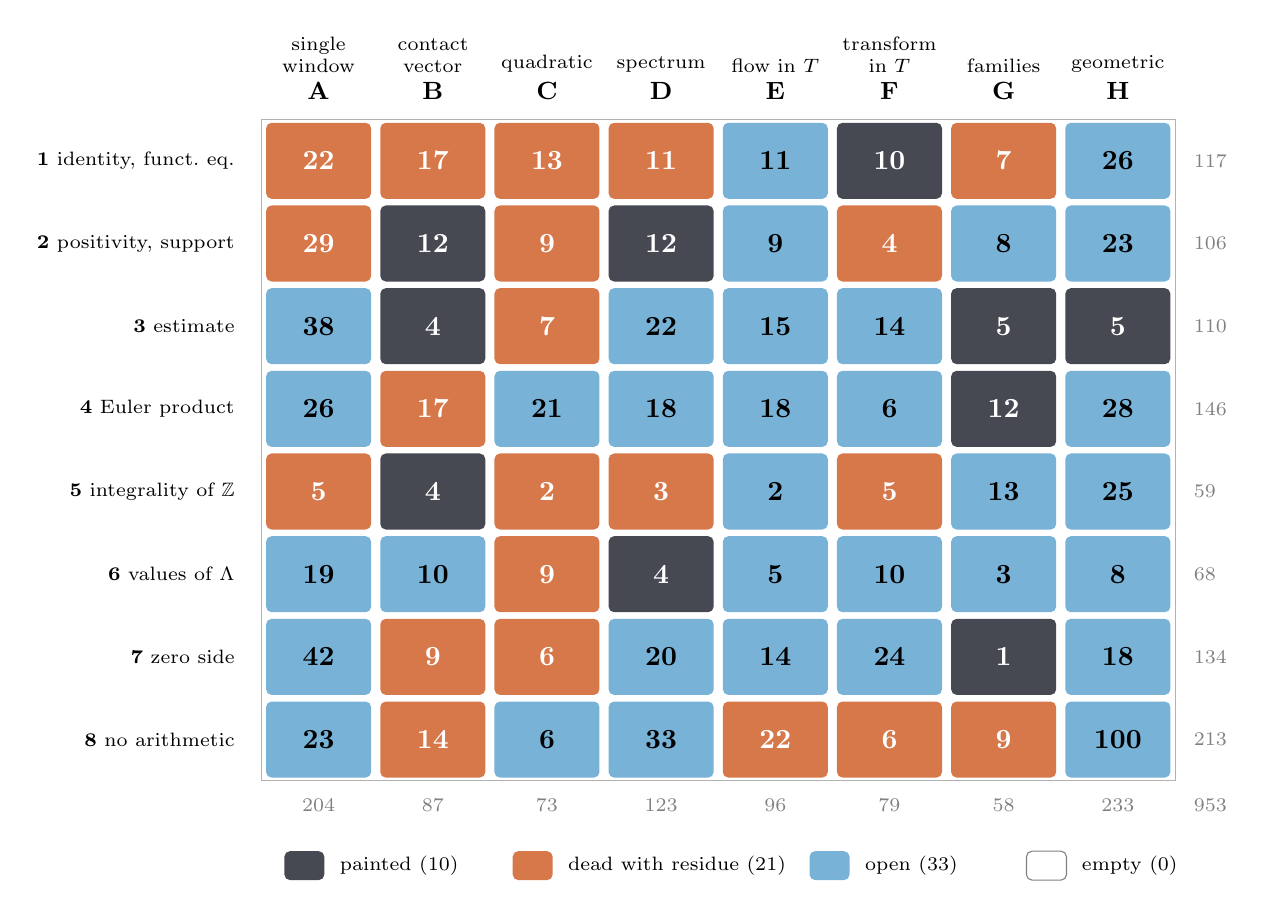
\begin{tikzpicture}[x=1.45cm,y=1.05cm,font=\small]
 % column labels
 \foreach \c/\lab [count=\i from 0] in {A/single window,B/contact vector,C/quadratic,D/spectrum,E/flow in $T$,F/transform in $T$,G/families,H/geometric}{
   \node[anchor=south] at (\i+0.5,0.12) {\textbf{\c}};
   \node[anchor=south,font=\scriptsize,text width=1.4cm,align=center] at (\i+0.5,0.45) {\lab};
 }
 % row labels
 \foreach \r/\lab [count=\j from 1] in {1/{identity, funct.\ eq.},2/{positivity, support},3/estimate,4/Euler product,5/integrality of $\Z$,6/values of $\Lambda$,7/zero side,8/no arithmetic}{
   \node[anchor=east,font=\scriptsize] at (-0.15,-\j+0.5) {\textbf{\r}\ \lab};
 }
 % data: status P painted, R residue, O open
 \foreach \row [count=\j from 1] in {
   {R/22,R/17,R/13,R/11,O/11,P/10,R/7,O/26},
   {R/29,P/12,R/9,P/12,O/9,R/4,O/8,O/23},
   {O/38,P/4,R/7,O/22,O/15,O/14,P/5,P/5},
   {O/26,R/17,O/21,O/18,O/18,O/6,P/12,O/28},
   {R/5,P/4,R/2,R/3,O/2,R/5,O/13,O/25},
   {O/19,O/10,R/9,P/4,O/5,O/10,O/3,O/8},
   {O/42,R/9,R/6,O/20,O/14,O/24,P/1,O/18},
   {O/23,R/14,O/6,O/33,R/22,R/6,R/9,O/100}}{
   \foreach \s/\n [count=\i from 0] in \row {
     \if\s P\def\fc{cDead}\def\tc{white}\fi
     \if\s R\def\fc{cRes}\def\tc{white}\fi
     \if\s O\def\fc{cOpen}\def\tc{black}\fi
     \fill[\fc,rounded corners=2pt] (\i+0.04,-\j+0.04) rectangle (\i+0.96,-\j+0.96);
     \node[text=\tc,font=\bfseries] at (\i+0.5,-\j+0.5) {\n};
   }
 }
 % grid frame
 \draw[gray!60,line width=0.3pt] (0,0) rectangle (8,-8);
 % column totals
 \foreach \t [count=\i from 0] in {204,87,73,123,96,79,58,233}
   \node[font=\scriptsize,gray] at (\i+0.5,-8.3) {\t};
 \foreach \t [count=\j from 1] in {117,106,110,146,59,68,134,213}
   \node[font=\scriptsize,gray,anchor=west] at (8.08,-\j+0.5) {\t};
 \node[font=\scriptsize,gray,anchor=west] at (8.08,-8.3) {953};
 % legend
 \begin{scope}[shift={(0.2,-9.2)}]
   \fill[cDead,rounded corners=2pt] (0,0) rectangle (0.35,0.35); \node[anchor=west,font=\scriptsize] at (0.4,0.17) {painted (10)};
   \fill[cRes,rounded corners=2pt] (2.0,0) rectangle (2.35,0.35); \node[anchor=west,font=\scriptsize] at (2.4,0.17) {dead with residue (21)};
   \fill[cOpen,rounded corners=2pt] (4.6,0) rectangle (4.95,0.35); \node[anchor=west,font=\scriptsize] at (5.0,0.17) {open (33)};
   \draw[gray,rounded corners=2pt] (6.5,0) rectangle (6.85,0.35); \node[anchor=west,font=\scriptsize] at (6.9,0.17) {empty (0)};
 \end{scope}
\end{tikzpicture}
\caption{The $8\times8$ grid of routes for row D. Rows: how the $\zeta$-specific datum enters
(Definition~\ref{def:rows}); columns: what object carries the argument (Definition~\ref{def:cols}).
The number in each cell is the number of routes placed there; grey margins are row and column totals. Snapshot of the record at phase 163 (953 routes); the current totals (1022 routes, phases 164--167) are given in the text and in the record's master grid, with no change of cell status except $6D$, $5G$ and $7C$.}
\label{fig:grid}
\end{figure}

\subsection{How to read the grid}
Three features stand out.

\emph{The painted cells lie on the prime-side/estimate block and on the families column.} Row 2 (positivity
and support) is painted in columns B and D: whatever uses only $a\ge0$ and prime support at the contact
vector or in the spectrum is killed by deletion and the $\kappa$-models (wall W3). Column G is painted in
rows 3, 4, 7 by the method theorems (W9) and the rationality wall (W8); cell $5G$, painted until phase 163, is open again with the Beurling frontier (\S\ref{subsec:beurling}). Row 3 is painted in B, G, H:
estimates have nothing to say linearly at the contact, or through families, or through geometry,
because of Theorem~\ref{thm:M}.

\emph{The open cells are concentrated in rows 4--8 and in columns A, E, H.} This does not mean that these
cells contain promising routes. Most open entries in columns A, E and H are unbuilt objects or pending
audits, and many will fall to E1. ``Open'' means only that a precise statement is unsettled.

\emph{Row 6 is open except at $6C$.} Apart from the Selberg difference channel ($6C$, closed with the
witness-parity residue by rounds 23--24), no cell in which the exact identity $\Lambda*1=\log$ is used at
the sign step is closed. Together with row 5, which is open in E and H, this is the region singled out by the
specification of \S\ref{sec:spec}: an argument that separates $\zeta$ from Beurling--DMV and from $\Lambda\chi_2$
at once must use integrality \emph{and} exact values, and those are rows 5 and 6.

\subsection{The residues of the closed cells}
For the twenty-one cells dead with residue the residue is a single precise statement. Examples:
$1B$: the global Sonin range condition at first contact (an equivalent of Problem~17.7 of
\cite{Paper47}, hence an E1 sink for columns B and C); $1C$: a scalar terminal target
$X_T=\frac12\|(I+\varepsilon C_{\log})g\|^2$ not realised from the finite identities; $2F$: complete
monotonicity (a Bernstein property) of $T\mapsto\lamA$ or of a transform of it; $5A$: the class-dependent
value bound (Problem~A of \cite{Paper47}); $5D$: the Smith normal form of the Gram matrix of the contact
vector over $\Z$; $7B$: a uniqueness statement for a boundary-rigidity system not yet audited;
$8E$: fixed-level convergence of a flow whose endpoint fails at the critical extreme. The four cells
closed in rounds 22--24 have residues $8B$, $5C$: asymmetric node weighting, i.e.\ a signed $Z'/Z$ at the
Gauss nodes (zero side, O2201.1); $6C$: the parity of the witness (OS-2); $5F$: non-vanishing of one
exterior Tate scalar $c_f$ on the radical from integrality (O2302.2). The cell $1D$, closed in rounds 27--28, keeps the residue of recomputing the boundary triple of the prolate form (deficiency $(4,4)$, see Remark~\ref{rem:r2728}) and a comparison with Burnol, both neutral with respect to RH.

\section{The universal walls}\label{sec:walls}

The walls W1--W12 are the mechanisms which kill routes in at least three cells. Each is stated as a
theorem (when the statement is a proved result about $\zeta$ or about the forms), or as a meta-theorem
(when it is a statement about a class of arguments, proved by exhibiting the reduction uniformly on the
class). The cells a wall paints are those in which it is the killer of record.

\begin{metatheorem}[W1: restatement]\label{W1}
Let $\mathcal R$ be an argument whose sign step is an equality of the form ``positivity of $X$'' where $X$
is one of: a Kre\u{\i}n or de Branges structure attached to the window data; a Herglotz function built
from $\xi'/\xi$; the Li or Keiper coefficients; Nyman--Beurling completeness; the global Sonin range at a
first contact; a per-window law quantified over all $T$; the flat-top certificate of
Theorem~\ref{thm:Z}; a Hodge-index inequality on a correspondence surface. Then the statement is
equivalent to RH, and $\mathcal R$ is a reformulation.
\end{metatheorem}
\noindent\emph{Paints} $1A$, $1B$, $1E$, $1F$, $2B$, $2E$, $2F$, $3F$, $7A$, $7E$, $7F$, $7H$, $8A$, and it is the
killer of roughly $40\%$ of all dead routes. The equivalences are classical (Li, Bombieri--Lagarias
\cite{BombieriLagarias1999}, Nyman--Beurling, de Branges, Lagarias' Herglotz criterion) or proved in
\cite{Paper47}: the certificate theorem (Theorem~\ref{thm:Z}) and the Kre\u{\i}n indeterminacy
reformulation \cite[Thm.~8.5]{Paper47}. One instance proved in the record: the generating
function $\Phi(s)$ of the window family over all $T$ is, for $s>\frac12$, a Poisson factor times
$2\Rel\xi'/\xi$, so its positivity is Lagarias' criterion and the first contact is invisible in it.

\begin{theorem}[certificate = explicit formula; \protect{\cite[Thm.~7.2]{Paper47}}]\label{thm:Z}
Every certificate of the complete form at window $T$ in the dual program is, up to an arbitrarily small
correction, the explicit formula evaluated on $w(u)\cos(\tau u)$ for a flat-top weight $w\equiv1$ on
$[-2T,2T]$; and RH holds if and only if, for every $T$, the function $\sum_\rho\widehat w(\tau-\gamma_\rho)$
admits such a nonnegative one-sided smoothing.
\end{theorem}

\begin{theorem}[W2: the margin decays; Theorem M]\label{thm:M}
(a) \cite[Thm.~11.5]{Paper47}: $\lamW\le\lambda^{\mathrm P}_T\le\lamA\le\mathcal B(T,k)$ with an
explicit $\mathcal B$, and $\limsup_{T\to\infty}\lamA\le0$.
(b) For every $\varepsilon>0$ there is $T_0(\varepsilon)$ such that for $T\ge T_0(\varepsilon)$,
\[
\lamW\le\lambda^{\mathrm P}_T\le\lamA\le\exp\!\big(-e^{(2-\varepsilon)T}\big).
\]
\end{theorem}
\noindent Part (b) is proved unconditionally in the record (Appendix~\ref{app:index}); it is not yet part of a
refereed paper. The test vectors are truncations of the radical vectors $\Phi_F=P(z^2)\Xi(z)$ of the
extended form, whose tails are doubly exponentially small; the smallness is a density phenomenon and not
an arithmetic one. \emph{Consequence:} no argument that needs a margin, a compactness gap, a bootstrap or
a perturbation of size larger than $\exp(-e^{2T})$ at window $T$ can succeed. Averages over $T$ do not
imply per-window statements (the master-quantifier lemma of Paper~29), and per-window arithmetic has a
ceiling of order $T/\log T$.
\emph{Paints} $3A$, $3E$, $5A$, $7D$, $2D$, partly $3C$ and $8F$.

\begin{metatheorem}[W3: class blindness]\label{W3}
If the sign step of $\mathcal R$ uses only $a\ge0$, $\supp a\subset\{p^k\}$, the functional equation, or laws
that are monotone in the weights, then it holds for deletion, the $\kappa$-models, Davenport--Heilbronn,
Epstein and (uncertified) the Type I curve, and $\mathcal R$ proves a false statement.
\end{metatheorem}
\noindent The proof is by inspection that each such property is shared (Table~\ref{tab:falsifiers}) together with
\cite[Thm.~12.5]{Paper47}. Perron--Frobenius and Hellmann--Feynman arguments orient only the
bottom eigenvalue and belong here: $\kappa$-models in the same support class have first contacts.
\emph{Paints} $2A$, $2B$, $2D$, $2E$, $3B$, $8D$, $8E$, $1D$, $4A$.

\begin{metatheorem}[W3$'$: integer-frequency blindness]\label{W3prime}
In every class defined by integer frequencies ($\mathrm{Fr}\subset\N$), the functional equation with $\Gamma(s/2)$,
finite order and real coefficients (any conductor) there are members with off-line zeros and a $2$-periodic
modular theta series (the model $f_\chi$ of Table~\ref{tab:falsifiers}); at conductor $1$ the class is $\{c\zeta\}$
(Hamburger). Global integrality of the frequencies is therefore either sign-blind or an identification.
\end{metatheorem}
\noindent This is W3 extended to the integer-frequency class (record R163\_1001, \S5, Theorem~\ref{thm:O} below,
proved given the cited off-line zeros of $f_\chi$). Routes: R163\_113/114 (identification form), R162\_2601c/2801
($\zeta=\zeta$ form), R163\_901 (window form), R163\_1001 (deformation, theta periodicity, window Hamburger).
\emph{Paints} the routes of R163\_1001 in $5E$ and $5F$, and constrains $1G$ and $4G$.

\begin{theorem}[exact obstruction; record R163\_1001, Theorem~O]\label{thm:O}
Let $\mathcal X$ be the class of $f$ with real coefficients, a discrete frequency set $\mathrm{Fr}(f)\subset[1,\infty)$,
finite order with at most a pole at $s=1$, and $\Lambda_f(s)=\Lambda_f(1-s)$ for $\Lambda_f=(q/\pi)^{s/2}\Gamma(s/2)f$.
Then $\{f\in\mathcal X:\mathrm{Fr}\subset\N\}$ contains $f_\chi$, $\{f\in\mathcal X:q=1\}$ contains $f_t$, and
$\{f\in\mathcal X:\mathrm{Fr}\subset\N,\ q=1\}=\{c\zeta\}$. Hence every statement ``global integrality of frequencies
plus data shared with $f_t$ or with $f_\chi$ implies $(\star_{\mathrm{cell}})$ at the witness'' is either false or has
$\{c\zeta\}$ as its only model; in the second case integrality enters only as the identification $f=\zeta$. With the
Euler product at $q>1$ the class is the degree-one Dirichlet $L$-functions, where a mechanism would be GRH in degree
one, uniform in $\chi$. (PROVED given the off-line zeros of $f_\chi$.)
\end{theorem}

\begin{metatheorem}[W-identification]\label{Wident}
Every global property that separates $\zeta$ from all the falsifiers identifies $\zeta$: the class it defines is $\{\zeta\}$
(or $\{c\zeta\}$), and the question about off-line zeros returns unchanged as RH. Instances: Hamburger's theorem, Theorem~\ref{thm:O},
Theorem~\ref{thm:R}; the full list is Theorem~\ref{thm:ident}.
\end{metatheorem}
\noindent Record R164\_190 (synthesis of round 2 of phase 164). \emph{Paints} every class route of the record; in particular the
positive-tail route of $4F$ (records R164\_102, R164\_401) and the class readings of $1G$, $5E$, $5F$, $5G$, $7B$.

\begin{metatheorem}[W4: orientation]\label{W4}
If the sign step of $\mathcal R$ is invariant under $A_M\mapsto-A_M$, in particular if it is a quadratic
estimate of the finite sum--product (Poisson--Chebyshev) identity, then it cannot orient the sign. The
square of the sum$\times$product identity contains the square of the truncated Weil form; the sawtooth of
the floor function is the comb of (PC); unconditional positivities give lower bounds.
\end{metatheorem}
\noindent \emph{Paints} $4A$, $5A$, $5B$, $6B$, $3D$, $4C$, $2C$, $8B$.

\begin{metatheorem}[W5: jets at $\lambda=0$]\label{W5}
If the $\zeta$-specific input enters the sign step only as $\lambda\cdot(\dots)$ or as a first variation at
the contact, then it vanishes at $\lambda=0$ and gives nothing. Example (proved in the record): under
compression $P_TZ_PP_T=Z_T$ the Tate jets enter only as $\lambda\langle\Gamma_PF,\varphi\rangle$.
\end{metatheorem}
\noindent \emph{Paints} $1B$, $2B$, $4B$, $4C$, $6B$, $8B$.

\begin{metatheorem}[W6: linear limit]\label{W6}
Linear completions of the renormalised finite identities are tautological: the commutator identity
$[X,S_N]=-K_N$ holds, and the two finite equations (PC$+$) and (PC$-$) differ by an algebraic zero valid for
every source, so their linear content is one-dimensional.
\end{metatheorem}
\noindent The two identities are proved; the general exclusion of every linear-limit argument is
\emph{not} proved as stated, and we do not claim it. \emph{Paints} $1A$, $1B$, $6B$.

\begin{metatheorem}[W7: $\Lambda*1=\log$ used linearly]\label{W7}
If $\Lambda*1=\log$ enters the sign step linearly, it acts as a window translation $T\mapsto T+\frac12\log X$
or cancels at composite thresholds.
\end{metatheorem}
\noindent \emph{Paints} $6A$, $6B$, $6D$, $6E$ (as far as they are closed). This is why row 6 is open but no row-6
route has closed: the identity has only ever been used linearly.

\begin{theorem}[W8: finiteness; \protect{\cite[Thm.~7.11]{Paper47}}]\label{thm:finZ}
Let $Z\subset\R\setminus\{0\}$ be a finite symmetric multiset with $|Z|\ge2$ and $w$ even, continuous,
integrable, $w\equiv1$ on $[-2T,2T]$, $w\to0$ at infinity. Then $\sum_{\gamma\in Z}\widehat w(\tau-\gamma)$
takes negative values. In particular no finite set of zeros carries a flat-top certificate, and row D is
intrinsically infinite.
\end{theorem}
\noindent Together with the rationality wall (transport from finite fields meets the six-exponentials
obstruction), this \emph{paints} $1H$, $4G$, $7G$ and parts of $5H$, $2G$.

\begin{theorem}[W9: method theorems; \protect{\cite[\S\S18, 27]{Paper46}}]\label{W9}
(T1) A proof of row D must be uniform over number fields or name the property separating $\zeta$ from
$\zeta_K$. (T2) The axioms A1--A6 of the analytic frame are satisfied by an Epstein zeta function with
zeros off the line; hence the Euler product (A7--A9) must be used. (T5) No Parseval-type moment bound
extracts a single fibre from a family beyond the trivial bound.
\end{theorem}
\noindent \emph{Paints} $1G$, $2G$, $3G$, $4G$, $8G$.

\begin{metatheorem}[W10: absent carrier]\label{W10}
Every geometric or cohomological carrier proposed in the record either postulates the positivity or is
equivalent to RH. Specifically: a single pole forces at most one pair; a zero-side mechanism blind to
off-line blocks cannot see a failure; no $h^0$ with the required three properties exists, not even over
$\mathbb F_q$ (the frame defect theorem of Paper~46).
\end{metatheorem}
\noindent \emph{Paints} $2H$, $4H$, $5H$, $7H$, $8H$ (as far as they are closed).

\begin{metatheorem}[W11: one side at a time]\label{W11}
Unconditional positivity in the record is either purely prime-side or purely archimedean; every statement
coupling both is equivalent to RH. The archimedean part alone is not positive beyond a short range:
the archimedean complete form is negative from $T=0.4608$ \cite[Prop.~10.7]{Paper47}, and the archimedean
primitive form fails from $T\in(0.58,0.60)$ on \cite[Thm.~12.5(i)]{Paper47}.
\end{metatheorem}
\noindent \emph{Paints} $2A$, $4A$, $6H$, $8H$.

\begin{metatheorem}[W12: identity without sign]\label{W12}
Chains of exact identities (secular equations, Kato expansions, cofactor and Jacobian identities, the
Selberg--virial identity $\Lambda\log+\Lambda*\Lambda=\mu*\log^2$ in the virial functional) retain all the
information and carry no sign. The locality--phase--sign trilemma: an argument cannot be local, phase-exact
and signed at once; the gamma factor dominates every local balance.
\end{metatheorem}
\noindent \emph{Paints} $4B$, $4D$, $4E$, $8A$, $1H$.

\begin{remark}[weights]
In order of the number of routes killed: W1 $\gg$ W2 $>$ W3 (with W3$'$) $>$ W10 $>$ W9 $>$ W8 $>$ W4, W5.
\end{remark}

\section{A specification of a closing argument, and six problems}\label{sec:spec}

\subsection{The specification}
Reading the walls backwards gives necessary conditions. Each item is the contrapositive of a wall or of a
proved no-go.

\begin{condition}\label{spec}
An argument proving $\lamA\ge0$ for all $T$ (equivalently, excluding a first contact) must:
\begin{enumerate}
\item[S1] use $\lambda=0$ at the contact non-perturbatively, with no jet $\lambda\langle\cdot,\cdot\rangle$ (W5, F1);
\item[S2] be non-linear and non-polynomial in the test (a polynomial functional collapses to the Sonin
 range, linear integrality is Poisson summation);
\item[S3] not be orientation invariant: contain neither the square of (PC) nor the square of the truncated
 Weil form (W4);
\item[S4] separate $\zeta$ from every model of Table~\ref{tab:falsifiers} simultaneously, in particular from
 Beurling--DMV and from $\Lambda\chi_2$; hence use integrality of $\Z$ and exact values together;
\item[S5] not be a per-window statement with a gap (Theorem~\ref{thm:M}) nor ``for all $T$'' of a per-window
 law (W1); it must be an object in $T$ that is not a reformulation;
\item[S6] not be Hecke-equivariant nor equivariant under window translations (W7);
\item[S7] let the Euler product enter before regularisation and after resummation of the functional
 equation (the regularised jet is invariant under finite modifications);
\item[S8] not be a weight-blind spectral criterion (the Type I curve);
\item[S9] be uniform over number fields or name the separating property (T1), and use A7--A9 (T2);
\item[S10] not require an $h^0$ with the three properties, nor a carrier that postulates positivity (W10);
\item[S11] couple primes and the archimedean place in a way that is not already RH (W11), hence pass through
 an intermediate statement strictly weaker than an equivalence;
\item[S12] depend neither on a finite set of zeros (Theorem~\ref{thm:finZ}) nor on a numerical margin
 (Theorem~\ref{thm:M}).
\end{enumerate}
\end{condition}

\subsection{The first-contact witness}
We recall the structure that a first contact would have, since Problem~\ref{prob:1} is built on it. The
following is proved in the record, conditionally on the existence of a complete first contact $T_c$
(which is equivalent to $\neg$RH).

\begin{proposition}[structure of a hypothetical first contact]\label{prop:witness}
Assume $\neg$RH, and let $T_c=\sup\{T:\lamW>0\}$ and $E_c=\ker W_{T_c}$. Then:
\begin{enumerate}
\item[(i)] \emph{(Blaschke invariance.)} Moving a non-real zero $w$ of $\Fh$ to $\bar w$ preserves $\|F\|$,
 the support in $I_T$, the form domain and $W_T$ (on $\PT$ also $\mathfrak a_T$); this holds for every window
 datum with real multiplier and conjugation-closed polar block, hence for $\zeta$ and all the models above.
\item[(ii)] $E_c$ is finite-dimensional; every nonzero element has convex support $[-T_c,T_c]$; each nonzero
 parity part of $E_c$ contains a real, parity-definite \emph{witness} $F$ whose transform $\Fh$ has only real
 zeros, of density $T_c/\pi$.
\item[(iii)] \emph{(Gauss nodes.)} For distinct real zeros $x\ne y$ of $\Fh$ the node tests
 $\widehat H_x=\Fh/(z-x)$ are $W_{T_c}$-orthogonal, and on their span
 $W_{T_c}(G)=\sum_xw_x|\widehat G(x)|^2$ with $w_x\ge0$, $w_x>0$ for all but at most $\dim E_c-1$ nodes.
\end{enumerate}
The same holds at the primitive first contact $T_*$ with $\PT$ in place of $L^2(\IT)$.
\end{proposition}

Proposition~\ref{prop:witness} gives a margin-free object: it is qualitative, it lives at a finite
window, and it does not pass to a limit. But (i) holds for every model, so the witness by itself is class
blind (W3): the arithmetic must be added.

\subsection{The torsion distribution}
For $d\ge1$ let $\nu_d=\frac1d\sum_{r\bmod d}\delta_{r/d}$ on $\R/\Z$, so $\widehat{\nu_d}(k)=\mathbf1_{d\mid k}$.
For $a$ with $a(1)=0$ define the distribution on $\R/\Z$
\begin{equation}\label{eq:Phi}
\Phi_a=\sum_{d\ge2}a(d)(\nu_d-\Leb),\qquad \widehat{\Phi_a}(k)=(a*1)(|k|)\ (k\ne0),\quad\widehat{\Phi_a}(0)=0,
\end{equation}
and let $\cL_p$ be the transfer operator of $x\mapsto px$, $(\cL_p\Phi)^\wedge(k)=\widehat\Phi(pk)$.

\begin{theorem}[the $\times p$ cocycle]\label{thm:cocycle}
(a) For every prime $p$, $\cL_p\Phi_\Lambda-\Phi_\Lambda=\log p\,(\delta_0-\Leb)$.
(b) Conversely, if $a(1)=0$ and the identity in (a) holds for every prime $p$, then $a=\Lambda$; if $a*1\ne\log$,
the identity fails at the least prime dividing the least $n$ with $(a*1)(n)\ne\log n$.
(c) For a Beurling system with $\mathcal N_B\not\subset\Z$ the distribution $\Phi_{\Lambda_B}$ is not defined.
\end{theorem}
\begin{proof}
(a) $\widehat{\Phi_\Lambda}(k)=\log|k|$, and $\log|pk|-\log|k|=\log p$ for $k\ne0$, while both sides vanish at
$k=0$. (b) The identity for all $p$ and $\widehat\Phi(\pm1)=0$ give $\widehat\Phi(k)=\log|k|$ by induction on the
number of prime factors of $k$; Möbius inversion gives $a=\mu*\log=\Lambda$. The failing prime is the same
induction read contrapositively. (c) $\nu_g$ requires $g\in\Z$.
\end{proof}

Theorem~\ref{thm:cocycle} is the $\times p$ form of $\Lambda*1=\log$, and it is \emph{discontinuous in the
support}: moving one index off $\Z$ destroys $\nu_d$. It separates $\zeta$ from Beurling--DMV (by (c)), from
$\Lambda\chi_2$ (fails at $p=2$), from deletion and the $\kappa$-models (fails at $p\in\{2,3\}$), and from
Davenport--Heilbronn. It is the only object in the record that satisfies S4. Two negative facts are
proved: \emph{band-limited tests read only primes}, i.e.\ for the trigonometric polynomial $h_F$ with
$\widehat{h_F}(k)=\sum_j\mu(j)w_F(|k|j)$ one has $\langle\Phi_a,h_F\rangle=\sum_da(d)w_F(d)$ for every $a$, so
the pairing is the prime term and does not see (a); and the pairing through the atom at $0$ alone
reproduces the Gamma-pole contribution and dies at the first-contact pole.

\subsection{Six problems and their status}
The ranking of the unpainted directions is by the number of conditions of Specification~\ref{spec} met by
construction, weighted by the existence of a concrete object and a falsifiable first lemma. Problems
\ref{prob:1}--\ref{prob:4} were attacked in rounds 22--24 of the record and are \textbf{resolved negatively};
the one-line reason and the surviving residue follow each statement. The class-level route to Problem~\ref{prob:5}
was resolved negatively in rounds 25--26, and the surviving residues converge to Problem~\ref{prob:6}, which is open.

\begin{problem}[Blaschke--torsion pairing; cells $5C\times5E$ and $8B$]\label{prob:1}
Let $T_*$ be a hypothetical primitive first contact and $F$ a real-rooted parity-definite witness
(Proposition~\ref{prop:witness}). Construct from $F$ a test $g_F$ on $\R/\Z$ that is \emph{not} band-limited,
depends non-linearly on $F$ through its real zeros (the Gauss nodes), and reads the torsion atoms $r/d$ with
$r\ne0$ of $\Phi_\Lambda$, such that
\[
\Psi_T(F):=\langle\Phi_\Lambda,g_F\rangle
\]
(1) vanishes identically, as a function of the data, exactly when the cocycle of Theorem~\ref{thm:cocycle}(a)
holds, that is, for a Beurling system with $\mathcal N_B\subset\N$, $\Psi\equiv0$ if and only if $a=\Lambda$;
(2) fails on a declared line for $\Lambda\chi_2$ and for deletion; and (3) is forced, at $T=T_*$, to have a sign
incompatible with the Gauss-node representation $W_{T_*}(G)=\sum_xw_x|\widehat G(x)|^2$, followed along the
residue window $T\mapsto T_*+\delta$ by a non-linear integrality law.
\end{problem}
\noindent \emph{Conditions met by design:} S2, S4, S5, S6, S12 (no margin: the witness is qualitative).
\emph{Risks:} S1 and S3 at the contact; E1 if the rigidity is read as a Herglotz property; the Type I curve
must be passed first (S8). \emph{First falsifiable lemma:} part (1).

\noindent\textbf{Status: resolved negatively.} Node tests and their finite products are Paley--Wiener, so they
read $\Phi_\Lambda$ only on the window comb (OS-1), the node measure is the determinate Kre\u{\i}n extension
(E1), and the minimal atomic object $\sum_xq_x(-\zeta'/\zeta)(s+ix)$ loses its atoms at $s=\frac12$ by
functional-equation reflection and node symmetry; $\Lambda\chi_2$ passes through a twisted cocycle.
\emph{Residue} (O2201.1): an asymmetric node weighting, i.e.\ a signed $Z'/Z$ at the nodes, which is zero side.

\begin{problem}[the difference channel at the edge; cell $6C$]\label{prob:2}
In the edge-trace identity at $\frac12\log mn$, the Selberg identity $\Lambda\log+\Lambda*\Lambda=\mu*\log^2$ sits in
the sum channel. Control the difference channel $|\sum_nw_nn^{it}|^2$ at the edge without resumming to the
zeros, or prove that every such control reduces to the zero side.
\end{problem}
\noindent Exact and non-linear, and separates the four prime-side classes (S4, S7). Risk: it is per window (S5,
Theorem~\ref{thm:M}), and naive resummation returns a known identity without sign.

\noindent\textbf{Status: resolved negatively.} The Selberg identity holds iff $a=\Lambda$ (recursively), but node
quadrature is exact on type $\le2T_c$, so the channel values are values of $W$ and $w_x\ge0$ is $W\ge0$; the
contacts $n\in[e^{T_c},e^{2T_c})$ invisible to the nodes enter only through a signless cross term, antisymmetric
in the parity of the witness. \emph{Residue} (OS-2): the parity of the witness.

\begin{problem}[$\times p$ rigidity against $W_T$; cell $5H$]\label{prob:3}
Decide whether measure rigidity for the $\times p$ action (or o-minimal counting of Pila--Wilkie type)
applied to $\Phi_\Lambda$ against non-band-limited tests constrains $W_T$ at a first contact.
\end{problem}
\noindent Meets S4, S6, and S9 through $\Z$.

\noindent\textbf{Status: resolved negatively.} The node sets and their $p$-families are not definable in an
o-minimal structure, Kronecker node images are never torsion for two primes, torsion lies on algebraic carriers,
and below $\log2$ the window data of $\zeta$ coincide with a two-atom model of finite torsion support: no
$\bar{\mathbb Q}$-variety is attached to $F$ (W10) and the rationality wall applies (W8). No residue in $5H$
from this direction.

\begin{problem}[a global object in $T$ with Euler before regularisation; cells $4F$, $5F$]\label{prob:4}
The local Weil limit with weak renormalisation on the primitive $L^2$ space is constructed, with the prime
number theorem remainder. Prove that its value vanishes and that it preserves the radical; or find a
non-linear global transform in $T$ in which the Euler product enters before regularisation and which does not
reduce to $\xi'/\xi$ or to the global Sonin range.
\end{problem}
\noindent Meets S5 and S7 by design. First check: non-reduction to the generating function of W1.

\noindent\textbf{Status: resolved negatively.} The limit vanishes identically modulo Tate on every primitive source,
because $\zeta(1-\rho)=0$ kills the atoms, and a finite-dimensional radical invariant under the Volterra operator is
zero, so radicality is equivalent to Gate~1. \emph{Residues} (O2302.2): non-vanishing of the exterior Tate scalar
$c_f$ on the radical from integrality; (O2302.1) the finite-$N$ remainder, of Li type.

\begin{problem}[finite multiplicity implies none; cells $8F$, $4E$, $7E$]\label{prob:5}
Prove the dichotomy: if the number $m$ of zeros off the line (counted in a fixed normalisation) is finite,
then $m=0$.
\end{problem}
\noindent One of the few intermediate statements not equivalent to RH (S11), and it uses the Euler product
three times (S7). Risk: no precedent in the literature; the finiteness half is of Lindelöf strength.

\noindent\textbf{Status: class-level route resolved negatively.} Under $m$ off-line quartets with maximal
excess $\beta^*$ one has $\lim_T T^{-1}\log(-\lamA)=2\beta^*<1$, against an unconditional floor of exponent one,
so the first-contact machinery and Theorem~\ref{thm:M} point in the same direction and do not clash. The finite
model $M_m$ (Table~\ref{tab:falsifiers}) shares every class-level property used by that machinery, so any
such argument proves the statement only by proving it for $M_m$, which is false. The refined version, that an
atomic prime comb excludes a finite exponential density, is false as posed: the positive atomic weights
$\tilde\Lambda$ reproduce that density. By Hamburger-type rigidity, within the atomic logarithmic-derivative class
the statement has no class content. \emph{Residue:} Problem~\ref{prob:6}.

\noindent\textbf{Cells $4D$ and $8D$.} The Gamma--Euler detector $-\zeta'/\zeta(2m+1)$ detects only Gamma moments;
a bounded faithful comparison with $W_T$ exists iff the kernel is trivial at fixed $T$, with norm $\gtrsim1/\lambda(T)$,
so uniformity is the rate law of Theorem~\ref{thm:M}; the nonlinear Euler data before regularisation form a positive
diagonal algebra, and the residue folds into an earlier one. In $8D$, $\mathfrak a_T=P_ISP_I$ for the full-line Weil
form $S=S_0-2\ell_+\ell_-$, no positive $S$ compresses to it, the semilocal carrier passes deletion, and the
Connes--Consani Sonin count $N(T)$ is nondecreasing with first jump at the first contact and limit twice the number
of off-line pairs; $\sup N<\infty$ is again finite multiplicity. Both directions are resolved negatively.

\begin{problem}[the convergent lemma O2601.1, sharpened: the discrete Beurling frontier; cells $5G$, $8F$, $8D$, $4D$, $7E$, $4F$]\label{prob:6}
Originally: find an individual property of the Euler product of $\zeta$, using the exact values of $\Lambda$
non-linearly, which bounds the number of zeros off the line and fails for deletion, for the finite models $M_m$ and
for the atomic weights $\tilde\Lambda$ of Table~\ref{tab:falsifiers}. After phase 163 (\S\ref{subsec:beurling}) the
problem is stated in the following sharpened form.
\begin{enumerate}
\item[$(\mathrm{BF}^{\mathrm{disc}}_\theta)$] Is there a threshold $\theta_0>0$
such that every \emph{discrete} Beurling generalised number system (integer prime multiplicities) whose integer
counting function satisfies $N(x)=\rho x+O(x^\theta)$ for some $\theta<\theta_0$ has all the zeros of its zeta
function in $\Rel s>\theta_0$ on the line $\Rel s=\frac12$?
\end{enumerate}
By Theorem~\ref{thm:BFdisc} (\S\ref{subsec:beurling}) the answer is \emph{negative} for every $\theta_0>\frac13$: for each
$\theta'\in(\frac13,\frac12)$ there is an unconditional discrete system with $N=\rho x+O(x^{\theta'})$ and a positive
proportion of zeros on $\Rel s=\frac{1+\theta'}2-\varepsilon'$. \textbf{The remaining range is $\theta\le\frac13$}, where the
variance of the random rounding diverges. The ordinary integers have $\theta=0$, so a positive answer at any $\theta_0\in(0,\frac13]$ still gives RH. In the extended class
(positive prime measures, not necessarily integer multiplicities) the answer is negative for every $\theta\in(0,1)$ by
the rescaled system $\zeta_\theta$ of \cite[\S6.1]{Broucke2024} (Proposition~\ref{prop:zetatheta}); every analytic
obstruction is therefore excluded (Proposition~\ref{prop:analyticnogo}), and a proof must use the integrality of the
prime multiplicities; the one integrality result about zeros known to us \cite[Rem.~7]{Revesz2023} forces zeros with
$\beta>\theta$ when $\theta<\frac12$, which is compatible with RH. On the part of the class comparable with $\N$ the statement is equivalent to RH
(Corollary~\ref{cor:finitepert}), so any new content lies with systems whose prime measure differs from that of
$\zeta$ on a set of abscissa $>\frac12$. Before Theorem~\ref{thm:BFdisc} the known discrete constructions with off-line zeros needed $\theta\ge\frac12$:
Diamond--Montgomery--Vorhauer for $\theta>\frac12$ \cite{DMV2006} (read through \cite{Broucke2024,BDV2020}),
Zhang at $N=kx+O(x^{1/2}\exp(c(\log x)^{2/3}))$ \cite{Zhang2007} (read through its zbMATH record), and Broucke's
floor-rounding at $\theta\ge\frac12$ \cite[Thm.~6.3]{Broucke2024}; the system of \cite{BDV2020} satisfies RH with
large oscillation of $N$. The two earlier sub-forms are recorded: (O2801.1) whether the generalised-integer measure of
$\zeta_0=\zeta/R$, $R$ the rational factor of $m$ off-line quartets, can be non-negative with all zeros real, is
resolved negatively in the record (R162\_2901: strict positivity fails for every $m\ge1$, and a positive Beurling
structure with RH exists after multiplying by a symmetric rational factor, so positivity gives no contradiction);
(O2802.1) a non-formal property of the integer ledger $b\equiv1$, uniform in $k\asymp\log x$ for the Piltz family,
remains open and is subsumed by $(\mathrm{BF}^{\mathrm{disc}}_\theta)$ at $\theta=0$.
\end{problem}
\noindent The sharpened form is a class statement which $\zeta$ satisfies with margin ($\theta=0$ against
$\theta_0$), so it is weaker than RH at an intermediate step (S11); by the class obstruction of $M_m$, by
Hamburger rigidity and by $\zeta_\theta$, no argument using only analytic or positivity properties of the class can
prove it, and by Theorem~\ref{thm:BFdisc} integer multiplicities alone do not prove it either for $\theta_0>\frac13$. Open for $\theta_0\le\frac13$.
\emph{Status after phase 166} (R166\_701, R166\_702): at $\theta=0$ two rigidity statements are PROVED (T3/T4: adding a prime $q$ keeps
$\theta=0$ if and only if the remainder is a bounded coboundary for $x\mapsto x/q$; $\N$ together with any real $q>1$ is never $\theta=0$;
novelty to be checked against Hilberdink 2012); the conjectures C1 (every $\theta=0$ system is $\zeta$ up to a finite Euler modification) and C2
(some $\theta=0$ system has an off-line zero) are OPEN, and if C1 holds then C2 is equivalent to the negation of RH. Position-tuned and
prime-replacement systems reproduce the barrier $\theta\ge\beta$ (Lemma PT). The problem stays two-sided below $\frac13$; as a route to
row D it fails requirement (N), since the count $N$ is blind to zeros.

\noindent\emph{Status after rounds 32--37 of phase 163.} Theorem~\ref{thm:O}: global integrality of the frequencies
identifies $\zeta$ at conductor $1$ and is sign-blind at every conductor $q>1$ (model $f_\chi$, wall W3$'$); it enters a
proof of $(\star_{\mathrm{cell}})$ only as the identification $f=\zeta$, after which the sign must come from the values of
$\Lambda$. Two properties proposed earlier as separators are removed: on-line abundance (Levinson--Conrey, positive or even
full proportion), because for DH-type linear combinations of Euler products $100\%$ of the zeros lie on the line,
conditionally on GRH and a pair-independence hypothesis \cite{BombieriHejhal1995}, while infinitely many lie off it
\cite{KaczorowskiKulas2007,SaiasWeingartner2009} (record R163\_602, F2); and Riemann--Siegel or approximate functional equation structure, which uses only the functional equation and
is shared by $f_\chi$ (record R163\_603). Two separators survive: (i) the \emph{Euler product above the window}, that is, the
tail $\mathcal T_X(x)=\sum_{n\ge X}\Lambda(n)n^{-1/2+ix}$, $X=e^{2T_c}$, of $-\zeta'/\zeta$, which carries every off-line
residue at a first-contact witness (record R163\_801, Theorem~3) and which the model $f_t$ does not share (phase 164,
the tail theorem (TC), record R164\_000); and (ii) $(\mathrm{BF}^{\mathrm{disc}}_\theta)$ for $\theta\le\frac13$, the only
formulation in the record in which integrality has content about zeros that is not identification.

\noindent\emph{Status after rounds 1--2 of phase 164.} Separator (i) is closed. Its kernel-equation reading through the hybrid
Euler--Hadamard cut is a restatement of the zero-side identity (record R164\_101, wall E1); a positive tail without the functional
equation is zero-blind (record R164\_102, Theorem~A); with the functional equation the positive witness class is $\{\zeta\}$
(Theorem~\ref{thm:R}). By Theorem~\ref{thm:ident} every separating class property identifies $\zeta$. What is left of (ii) is
the discrete frontier off the Witt lattice: within bounded-deviation roundings of the Witt counts the threshold $\frac13$ is real
(Remark~\ref{rem:onlynonident}). Problem~\ref{prob:6} for $\theta_0\le\frac13$ remains OPEN, and it is the only remaining
non-identification content.

\begin{remark}[rounds 27--28]\label{rem:r2728}
The Tate transfer system $2\times2$ of $4E$ gives the canonical system $H_S=\frac12\exp(2\Theta\sigma_1)$,
$\Theta=\sum_{p\in S}\operatorname{artanh}p^{-1/2}$, positive for every chain of boosts and identical for $M_m$: it is
RH-neutral (W12); the index count of phase 61 is uncertified and equals $0$ after normalisation. The
two-variable Weil form of $4C$ is closed by the index bridge of doc 108 (W2, E1). In $1D$, Fourier
anticommutation fails by an index count, and the invariants of the boundary triple of the prolate form depend
only on $(\lambda,2\pi)$, so they cannot touch Problem~\ref{prob:6} (W3); the hostile review found that the
deficiency is $(4,4)$, not $(2,2)$ ($\pm\infty$ are limit circle), so the boundary-triple computation is to be
redone, while the $\Lambda$-freeness of the invariants stands. Two angles on Problem~\ref{prob:6}: quantitative
Hamburger rigidity returns $c\,\zeta R$ for every $m$, and integer-$k$ Piltz sums see only the pole (under finitely
many off-line zeros the Lindel\"of hypothesis holds), which leave O2801.1 and O2802.1. All residues of the grid now
converge to Problem~\ref{prob:6}. Remaining unattacked: $5E/5F$ (non-linear integrality); $6D/6A$ and O2801.1 were
in progress (settled in round 29, \S\ref{subsec:beurling}).
\end{remark}

\begin{remark}[ranking after rounds 25--26]
The directions $8F$, $4D$ and $8D$ are resolved negatively, and their residues converge to Problem~\ref{prob:6}.
The remaining unattacked items are: non-linear integrality in $T$ ($5E/5F$); the Tate transfer system $2\times2$ ($4E$);
the structural identities at $\log2$ ($6D/6A$); Fourier anticommutation and the two-variable Weil form ($1D$, $4C$).
\end{remark}

\begin{remark}[residues and ranking after rounds 22--24]
After rounds 22--24 the ranking was: Problem~\ref{prob:5} ($8F/4E/7E$); a Gamma--Euler detector (below, $4D$);
the operator compression of $8D$; non-linear integrality followed in $T$ (O1802.3 together with O2302.2, cells
$5E/5F$); and the never-attempted Tate transfer system $2\times2$ in $4E$. New residues, unattacked:
O2201.1 ($8B$, $5C$, zero side), OS-2 ($6C$), O2302.1--2 ($5F$), O2202.1 (primitive form of the node
identity, $6B$), O2401.1 (individual sizes of the visible and hidden parts at the margin, $7D$).
\end{remark}

\begin{remark}[ranked but not stated, before rounds 25--26]
Next in rank (the first two now resolved negatively, above): a Gamma--Euler detector $-\zeta'/\zeta(2m+1)$ which is faithful but lacks a primitive
comparison with $W_T$ (cell $4D$); $\mathfrak a_T$ as the compression of an explicit self-adjoint operator
together with the Connes--Consani Sonin count (cell $8D$); and inexpensive structural identities at
$T=\log2$ (cells $6D$, $6A$), which are tools, not closing arguments. Excluded by the specification:
$7D$ (Theorem~\ref{thm:M}, S5), $3C$ (E1), de Bruijn--Newman monotonicity of the Kre\u{\i}n index in $1E$
(W3), the six-clause adelic object in $2G$ (W10), and certificates in $3A$ (S12).
\end{remark}

\subsection{The Beurling frontier (round 29 and phase 163)}\label{subsec:beurling}
We record the statements behind the sharpened Problem~\ref{prob:6}. A \emph{Beurling system} in the extended
sense is a pair of non-decreasing functions $\Pi,N$ on $[1,\infty)$ with $dN=\exp_*(d\Pi)$; it is \emph{discrete} if
$d\Pi=\sum_j\sum_k k^{-1}\delta_{p_j^k}$ for a multiset of primes $p_j>1$. Proofs are in the record (R163\_101,
R163\_102, R163\_190, R163\_191); statements labelled \emph{cited} rest on the references read there.

\emph{The canonical exchange.} For an off-line quartet $\frac12\pm\delta\pm i\gamma$ put $w=s-\frac12$ and
$E_{\delta,\gamma}=[((w-\delta)^2+\gamma^2)((w+\delta)^2+\gamma^2)]/(w^2+\gamma^2)^2$. The product $E$ over all quartets
converges normally away from its poles, $\log E(\frac12)=2\sum\log(1+\delta^2/\gamma^2)$, and
$d\Pi_{\zeta/E}=d\Pi_\zeta+q_E$ with $q_E$ an explicit distribution. The statement ``the exact arithmetic of $\zeta$
forces $q_E=0$'' is equivalent to RH: $q_E$ is the difference between each quartet's contribution to the explicit
formula and that of its projection onto the line (E1). If $\nu_N=\nu_0*\kappa$ with $\nu_0,\kappa\ge0$ both with
unit mass at $0$, both are supported on $\log\N$; but $E(\sigma)<1$ for large real $\sigma$ in a finite exchange, and
the example $K(s)=1-c/(s+1)$ shows that exact integers, the Euler product and a positive quotient do not force a
trivial factor.

\begin{proposition}[extended class; this is Broucke's own system \cite{Broucke2024}, cited, not new]\label{prop:zetatheta}
For $\theta\in(0,1)$ the system with $dN_\theta=\sum_nn^{\theta/(1-\theta)}\delta_{n^{1/(1-\theta)}}$ is a Beurling
system in the extended sense with zeta function $\zeta((s-\theta)/(1-\theta))$, $N_\theta(x)=(1-\theta)x+O(x^\theta)$, and
infinitely many zeros on $\Rel s=\frac{1+\theta}2$.
\end{proposition}

\begin{proposition}[analytic NO-GO]\label{prop:analyticnogo}
No argument that uses only analyticity of $\zeta_B-\rho/(s-1)$ in $\Rel s>\theta$, polynomial growth and
Phragm\'en--Lindel\"of bounds, positivity of $d\Pi$ (Landau), Jensen counts, an Euler product in the extended sense,
or the zero-density bounds of \cite{Broucke2024}, proves a zero-free region to the right of $\Rel s=\frac{1+\theta}2$
for systems with $N=\rho x+O(x^\theta)$ that contains the line $\Rel s=\frac{1+\theta}2$ (that is, that there are no
zeros with $\Rel s\ge\frac{1+\theta}2$). In particular any theorem ``$\theta<\frac12$ implies RH'' uses integer prime
multiplicities.
\end{proposition}

\noindent Integrality does constrain zeros. By a remark of R\'ev\'esz \cite[Rem.~7]{Revesz2023}, resting on a result
of Hilberdink \cite{Hilberdink2010} (cited, primary not read), a discrete system with $N=\rho x+O(x^\theta)$ and
$\theta<\frac12$ must have zeros with real part $\beta>\theta$. This is consistent with RH, with
Proposition~\ref{prop:zetatheta} and with Conjecture $C_{1/3}$ below: it pushes zeros to the right of $\theta$, not onto
the line. Whether it can be sharpened towards the line is part of Problem~\ref{prob:6}.

\begin{lemma}[rational modifications]\label{lem:ratmod}
If $\zeta R$, with $R$ rational and $R(\infty)=1$, is a positive Beurling system with a simple pole at $1$ and
$N=\rho x+O(x^\theta)$, and $R$ vanishes at $\frac12+\beta+i\gamma$ with $\beta>0$, then $\theta\ge\frac12+\beta$.
\end{lemma}

\begin{theorem}[lattice rigidity]\label{thm:latticerig}
If a discrete system has $N(x)=\lfloor x\rfloor+c$ for all large $x$, then $c=0$, its integers are $\N$ with
multiplicity one and its primes are the ordinary primes.
\end{theorem}

\noindent Rigidity fails one step later: if $\zeta_B=\zeta A$ with $A=\sum a_mm^{-s}$ a generalised Dirichlet series and
$\sum|a_m|<\infty$, then $N_B=A(1)x+O(1)$ (Lemma S of the record); finite deletions and root substitutions give
non-lattice discrete systems with bounded error.

\begin{theorem}[zero transfer]\label{thm:zerotransfer}
Let $B$ be a Beurling system with $N_B=\rho x+O(x^\theta)$, $\rho>0$, $\theta<1$; write $\Pi_B=\Pi_\zeta-\tau+q$ with
$\tau=(\Pi_\zeta-\Pi_B)^+$, $q=(\Pi_B-\Pi_\zeta)^+$, and let $\sigma_\tau$ be the abscissa of convergence of
$\int x^{-s}d\tau$. In $\sigma>\max(\sigma_\tau,\theta,0)$ the zeros of $\zeta_B$ and of $\zeta$ coincide with multiplicity.
\end{theorem}

\begin{corollary}[finite perturbations]\label{cor:finitepert}
If $B$ is obtained from $\N$ by deleting finitely many primes and adding a multiset $Q$, and $N_B-\rho x$ is bounded,
then $Q$ is finite with $|Q|$ at most the number of deleted primes, and $\mathrm{RH}_B\iff\mathrm{RH}$. More generally,
every system with $\sigma_\tau\le\frac12$ and error $O(x^{1/2})$ has the zeros of $\zeta$ in $\sigma>\frac12$: there is no
perturbative counterexample to $(\mathrm{BF}^{\mathrm{disc}}_0)$.
\end{corollary}

\emph{Random rounding.} Rounding the multiplicities of $\zeta_\theta$ randomly to $\lfloor a\rfloor$ or
$\lceil a\rceil$ with mean $a$ keeps the zeros of $\zeta_\theta$ in $\sigma>\frac{1-\theta}2$ and gives integer error of
exponent $\max(\theta,\frac{1-\theta}2)$ once the full $\exp_*$ chaos is controlled. Deterministic floor-rounding
\cite[Thm.~6.3]{Broucke2024} fails below $\frac12$ because its error is bounded by total variation; random rounding
replaces it by an $\ell^2$-type bound. The control of the chaos was conjectured in an earlier version of this paper
(Conjecture $C_{1/3}$) and is now a theorem (record R163\_803, hostile pass R163\_891 ``valid with fixes'', fixes applied).

\begin{theorem}[Beurling frontier, discrete, unconditional]\label{thm:BFdisc}
Fix $\theta\in(\frac13,\frac12)$. There is a discrete Beurling system $\mathcal P$, constructed at random, with the
following properties almost surely. Its generalised primes and integers have non-negative integer multiplicities, and
\begin{enumerate}
\item[(i)] $N_{\mathcal P}(x)=\rho x+O_\varepsilon(x^{\theta+\varepsilon})$ for every $\varepsilon>0$, with $\rho>0$;
\item[(ii)] $\zeta_{\mathcal P}$ extends meromorphically to $\sigma>\frac{1-\theta}2$, and its zeros there are exactly the points
$\theta+(1-\theta)\varrho$, $\varrho$ running over the non-trivial zeros of $\zeta$, with the same multiplicities;
\item[(iii)] in particular $\zeta_{\mathcal P}$ has a positive proportion of its zeros on $\Rel s=\frac{1+\theta}2>\frac12$ (Hardy, Selberg).
\end{enumerate}
Consequently, for every $\theta'\in(\frac13,\frac12)$ the implication ``$N=\rho x+O(x^{\theta'})\Rightarrow$ Beurling RH'' fails in
the discrete class (take $\theta<\theta'$), and Broucke's density range $\alpha>\frac{1+\theta'}2$ \cite{Broucke2024} is optimal for
discrete systems up to an arbitrarily small loss in $\theta'$.
\end{theorem}

\begin{proof}[Proof sketch]
Put $a=\theta/(1-\theta)\in(\frac12,1)$ and $w=(s-\theta)/(1-\theta)$. For $q>1$ the necklace polynomials
$c_k(q)=k^{-1}\sum_{d\mid k}\mu(k/d)q^d$ satisfy $(1-qz)^{-1}=\prod_k(1-z^k)^{-c_k(q)}$ for $|z|<1/q$; $c_k(q)\ge0$ for $q\ge2$,
and for $1<q<2$ only finitely many $c_k(q)$ are negative. With $q_p=p^a$ and $z=p^{-(w+a)}$, so that $q_pz=p^{-w}$, the
system with $c_k(p^a)$ primes at the points $p^{k/(1-\theta)}$ has zeta function $\zeta(w)$, which is $\zeta_\theta$. Round
independently: $b_{p,k}\in\{\lfloor c^+_{p,k}\rfloor,\lceil c^+_{p,k}\rceil\}$ with mean $c^+_{p,k}=\max(c_{p,k},0)$, and take
$b_{p,k}$ primes at $p^{k/(1-\theta)}$. All products of primes are again of the form $n^{1/(1-\theta)}$, so
\begin{gather*}
\zeta_{\mathcal P}(s)=\zeta(w)\,F(w)\,G(w),\qquad F=\prod_{c_{p,k}<0}(1-p^{-k(w+a)})^{-|c_{p,k}|},\\
G=\prod_{p,k}(1-p^{-k(w+a)})^{-\varepsilon_{p,k}},\qquad \varepsilon_{p,k}=b_{p,k}-c^+_{p,k}\in(-1,1),
\end{gather*}
with $F$ a finite product and $FG=\sum_n\gamma_nn^{-w}$ a random \emph{multiplicative} function whose values at distinct
rational primes are independent, $\mathbb E\gamma_p=0$, $|\gamma_{p^j}|\le C_\eta(1+\eta)^jp^{-ja}$. (i): the exact identity
$N_{\mathcal P}(x)=\sum_{m\le X}g_mS_a(X/m)$, $X=x^{1-\theta}$, $S_a(Y)=\sum_{d\le Y}d^a$, and Euler--Maclaurin for $S_a$ reduce
(i) to $\sum_{m\le Y}\gamma_m\ll Y^\varepsilon$ and one weighted variant, almost surely. The $2q$-th moment of
$\sum_mc_m\gamma_m$ ($|c_m|\le1$) is bounded by an Euler product in which the $E=1$ terms vanish by $\mathbb E\gamma_p=0$ and the
$E\ge2$ terms contribute $\ll\sum_pp^{-2a}<\infty$ exactly because $2a>1$, that is $\theta>\frac13$; Chebyshev and Borel--Cantelli
finish. (ii)--(iii): $\log G=L+R$ with $L=\sum_p\varepsilon_{p,1}p^{-a-w}$ a Dirichlet series with independent, bounded, mean-zero
coefficients and summable variances for $\Rel w>\frac12-a$, hence almost surely convergent there (Kolmogorov's one-series
criterion, Jensen--Cahen), and $R$ absolutely convergent there. So $FG$ is analytic and zero-free in $\Rel w>\frac12-a$, which
is $\sigma>\frac{1-\theta}2$ and contains no trivial zero of $\zeta(w)$. Full proof: record R163\_803.
\end{proof}

\begin{remark}[novelty and what is not claimed]\label{rem:BFnovelty}
Hilberdink's bound (every discrete system has $\max\{\alpha,\beta\}\ge\frac12$) and the remark of R\'ev\'esz
\cite[Rem.~7]{Revesz2023} are consistent with Theorem~\ref{thm:BFdisc}, whose zeros have real part $\frac{1+\theta}2>\frac12$.
The closest prior art known to us is Broucke--Debruyne--R\'ev\'esz \cite[Thm.~1.3]{BDR2023}, which constructs
$[\alpha,\beta]$-systems with integer error exponent $\beta<\frac12$ \emph{conditionally on RH}, in the region
$\frac12<\alpha<\frac23$, $2\alpha/(\alpha+2)\le\beta<\frac12$; the pairs $(\alpha,\beta)=(\frac{1+\theta}2,\theta)$ of
Theorem~\ref{thm:BFdisc} lie outside that region for every $\theta>\frac13$, and the theorem is unconditional. The same paper
remarks that discrete examples with $\beta<\frac12$ must be built ``right from the start'' rather than by discretising a
continuous system; the present construction does so by rescaling to $p^{k/(1-\theta)}$ and rounding independently over the
rational primes, not by the Diamond--Montgomery--Vorhauer method of random primes in short intervals. Not yet checked: the
full text of Diamond--Zhang \cite[Ch.~17]{DiamondZhang2016} and the works citing \cite{BDR2023}; no priority is claimed until
this is done (record R163\_892). The theorem concerns Beurling systems only, not $\zeta$: Row D is unchanged. At $\theta=\frac13$ the
variance diverges and the method stops; at $\theta=\frac12$ the Euler--Maclaurin step needs $a<1$ and is not covered.
\end{remark}

\noindent By Theorem~\ref{thm:BFdisc} the frontier of Problem~\ref{prob:6} is at $\theta_0\le\frac13$. (Dedekind zeta
functions of quadratic fields have lattice exponent $\frac13$; no link is claimed.)

\subsection{Identification (phase 164)}\label{subsec:identification}
Write $\mathsf C=\sum_{n\in\mathbb Z}\delta_n$ for the Dirac comb. For $f(s)=\int_{[1,\infty)}\lambda^{-s}\,dN(\lambda)$,
absolutely convergent for $\Rel s>1$ with $N(\{1\})=1$, let $m_f=\delta_0+N+\check N$ be the even theta measure on $\mathbb R$
($\check N$ the reflection of $N$). By the Hecke--Bochner dictionary (Riemann's proof run in both directions), $\pi^{-s/2}\Gamma(s/2)f$
has $\zeta$'s functional equation, its two simple poles and finite order if and only if $m_f$ is tempered and $\widehat{m_f}=m_f$
(record R164\_401, Lemma~1).

\begin{theorem}[positive-off-$\N$ rigidity; record R164\_401, Theorem~R]\label{thm:R}
Let $f$ be as above, and suppose (a) $N=N_\zeta$ on $[1,X)$ for some $X>1$; (b) $N\ge0$ on $[1,\infty)\setminus\N$; (c)
$\Lambda_f(s):=\pi^{-s/2}\Gamma(s/2)f(s)$ satisfies $\Lambda_f(s)=\Lambda_f(1-s)$, is holomorphic except for simple poles at
$s=1$ and $s=0$ with the residues of $\zeta$'s completion, $\mathrm{Res}_{s=1}\Lambda_f=1$ and $\mathrm{Res}_{s=0}\Lambda_f=-1$, and
$s(s-1)\Lambda_f$ has finite order. Then $f=\zeta$. (The residues must be those of $\zeta$: with $\mathrm{Res}_{s=1}\Lambda_f=r\neq1$
the window acquires the atom $(r-1)\delta_0$ and the sinc step below does not apply; hostile pass R164\_491, F3.)
\end{theorem}
\begin{proof}
By the dictionary $m:=m_f$ is self-dual, by (a) $m=\mathsf C$ on $(-X,X)$, and by (b) $m\ge0$ off $\mathbb Z$. Put
$\eta=m-\mathsf C$. Then $\widehat\eta=\eta$, $\eta=0$ on $(-X,X)$, and in the Jordan decomposition $\eta=\eta_+-\eta_-$ the
negative part $\eta_-$ is carried by $\mathbb Z\setminus(-X,X)$, since $\eta=m\ge0$ off $\mathbb Z$. Fix $0<a<\frac{X-1}2$ and
$\chi\in C_c^\infty(-a,a)$, put $\psi=\mathbf 1_{[-1/2,1/2]}*\chi$, supported in $(-\frac X2,\frac X2)$, and
$\varphi=\psi*\tilde\psi$ with $\tilde\psi(y)=\overline{\psi(-y)}$, supported in $(-X,X)$. Then $\widehat\varphi=|\widehat\psi|^2$
and $\widehat\psi(\xi)=\frac{\sin\pi\xi}{\pi\xi}\widehat\chi(\xi)$ vanishes on $\mathbb Z\setminus\{0\}$. Self-duality and the
gap give
$\int|\widehat\psi|^2\,d\eta=\langle\widehat\eta,\varphi\rangle=\langle\eta,\varphi\rangle=0$.
The $\eta_-$ part vanishes because $\widehat\psi=0$ on its support, so $\int\mathrm{sinc}^2|\widehat\chi|^2\,d\eta_+=0$ and $\eta_+$
is carried by $(\mathbb Z\setminus\{0\})\cup Z(\widehat\chi)$. Replacing $\chi$ by $e^{2\pi iby}\chi$ shifts $Z(\widehat\chi)$
(a countable set) by $b$; for $b$ outside the countable set $Z(\widehat\chi)-Z(\widehat\chi)$ the two zero sets are disjoint, so
$\eta_+$, and hence $m$, is carried by $\mathbb Z$. A self-dual tempered measure $\sum a_n\delta_n$ with $a_0=1$ has a
$1$-periodic Fourier transform, so $m$ is $1$-periodic and $a_n=1$ for all $n$: $m=\mathsf C$, $N=N_\zeta$, $f=\zeta$.
Full proof and falsifier checks: record R164\_401 (lead audit R164\_190).
\end{proof}
\noindent Hamburger's theorem is the case $\mathrm{supp}\,N\subset\N$; here positivity off $\N$ and a gap above $1$ replace
integer support, and the values $\Lambda(n)$, $n<X$, are not used. Consequently every positive Beurling system with a window of
$\zeta$ of any length, $\Gamma_{\mathbb R}$, $\zeta$'s functional equation, its poles and finite order is $\zeta$, and the
question ``is there such a system with an off-line zero?'' (record O164.101) is equivalent to $\neg$RH. The model $f_t$ escapes
exactly through (b): it has negative coefficients off $\N$ for every $t\ne0$. Novelty is not claimed: we have not found
Theorem~\ref{thm:R} in this form, but its ingredients are classical (Bochner 1951 and Chandrasekharan--Narasimhan 1961 for the
modular-relation dictionary, Hamburger for the integer-support case, Cohn--Elkies for the sinc/linear-programming device), it is
close in spirit to C\'ordoba's theorem on Dirac combs (1989) and to Kahane--Mandelbrojt (1958), and it is plausibly folklore.

\begin{theorem}[identification; synthesis, record R164\_190]\label{thm:ident}
Every global property in the record that separates $\zeta$ from all the falsifiers of Table~\ref{tab:falsifiers} identifies
$\zeta$, and the properties that do not identify do not separate:
\begin{itemize}
\item integer frequencies and the functional equation at conductor $1$: the class is $\{c\zeta\}$ (Hamburger; Theorem~\ref{thm:O}; records R163\_113, R163\_1001);
\item integer frequencies and the functional equation at conductor $q>1$: the class contains $f_\chi$, with off-line zeros (record R163\_1001);
\item a measure $\ge0$ off $\N$, a gap $(1,X)$, the functional equation and the poles of $\zeta$: the class is $\{\zeta\}$ (Theorem~\ref{thm:R}; record R164\_401);
\item Euler product, integer frequencies, conductor $1$: $\{\zeta\}$; at $q>1$ a mechanism would be GRH in degree one (record R163\_1001, Theorem~O.2);
\item on-line abundance, Riemann--Siegel structure, families and Parseval: not separating (records R163\_602 F2, R163\_603, phase 150);
\item a positive tail without the functional equation: zero-blind (records R164\_102 Theorem~A, R164\_101; the model $\zeta_\theta$);
\item integrality of multiplicities without the functional equation ($\mathrm{BF}^{\mathrm{disc}}_\theta$): content only for $\theta\le\frac13$, and the Witt lattice does not go below $\frac13$ (Theorem~\ref{thm:BFdisc}; records R163\_803, R164\_201, R164\_291).
\end{itemize}
Hence no class statement defined by these properties, true for the excluded falsifiers and different from RH for $\zeta$,
implies $(\star_{\mathrm{cell}})$: a proof of $(\star_{\mathrm{cell}})$ must use $\zeta$ individually, after identifying it, from the
comb and the explicit formula at all heights (equivalently, the tail form (TC) of record R164\_000). (PROVED as a synthesis of the
cited statements.)
\end{theorem}

\begin{remark}\label{rem:onlynonident}
The only remaining content in the record that is not identification is Problem~\ref{prob:6} below $\frac13$: discrete Beurling
systems with $\theta\le\frac13$ off the Witt lattice (record O164.201a). Within the lattice class of bounded-deviation roundings of
the Witt counts, the error is $\gg x^{\theta+\delta(\theta)}$, $\delta(\theta)=\theta(1-3\theta)/(5-3\theta)$, for every
$\theta<\frac13$ (record R164\_201, Theorem~L, after the hostile pass R164\_291); that any counterexample must lie off the
lattice is ARGUED only.
\end{remark}

\paragraph{Phase 164, rounds 3--4.} The remaining routes of phase 164 close as follows (labels from the lead audit R164\_190).
(i) \emph{Zero-side sinc} (record R164\_501, Theorem~SA, PROVED): every test $\ge0$ on $\mathbb R$ annihilated by the kernel
equation at the witness is a kernel square $\widehat H\widehat H^{\#}$ with $H\in E_c$; the nodes have the critical density
$T_c/\pi$, so no spare type is left for the sinc step of Theorem~\ref{thm:R} (which needed $X>1$), and the output is the circular
identity (killer E1). (ii) \emph{Spectral invariants are window data} (record R164\_502, Lemma~L1, PROVED): the compressed operator
$A_T$ depends only on the symbol on $(-2T,2T)$, so determinants, heat traces and moments see nothing above $e^{2T}$ (route DEAD).
(iii) \emph{Proposition~4} (record R164\_501, PROVED): for $\Psi_y=G^2\,y/(z^2+y^2)\ge0$ one has
$\sum_\rho\Psi_y(t_\rho)=\mathfrak A_y-G(iy)^2\mathcal T(iy)$ with $\mathcal T(iy)=\sum_{\log n\ge2T}\Lambda(n)n^{-1/2-y}>0$, the
first identity at the witness in which $\Lambda\ge0$ at all heights enters with a sign; it is an identity, and its off-line weight
is $y/\gamma_q^2$. (iv) \emph{Drop-term principle} (record R164\_601, Theorem~3.1, PROVED): every inequality obtained by discarding
a signed tail holds for the true zeros of $\zeta$ whatever they are, and excludes a quartet only together with a lower bound
independent of the other zero terms; that bound is $(\star_{\mathrm{cell}})$ weighted by a kernel $K$ (record O164.601.1).
(v) \emph{dlVP cap at the witness} (record R164\_601, Theorem~3.3): a test with properties (i)--(iii) of R164\_501 exists (the de la
Vall\'ee Poussin test mounted on $G^2$; O164.501.1 closed), but the Fej\'er cap and the archimedean term $\asymp\log\gamma_q$ leave
only $\frac12-\delta_q\le c/\log\gamma_q$ (wall W2/M). The positive direction of $\mathrm{BF}^{\mathrm{disc}}_\theta$ below $\frac13$
is at least as strong as RH together with quadratic GRH (record R164\_503). \emph{Every route of phase 164 returns to
$(\star_{\mathrm{cell}})$.}

\paragraph{Phase 165.} The critical-interlacing phase closes as follows (labels from the lead audit R165\_190).
(i) \emph{Detection} (record R165\_101, Theorem~Det$+$, PROVED with a clustering caveat): if $\rho^*=\frac12+\delta^*+i\gamma^*$ is a zero
off the line, then $\lamW<0$ for all $T\ge\tau(\rho^*)$, with
$\tau(\rho^*)\le T_L(\gamma^*)+\frac12\log(\pi/2)+o(1)$, where $T_L(\gamma)=\frac12\log(\gamma/2\pi)$ is the Landau window and
$\frac12\log(\pi/2)=0.2258$. Proof idea: divide $\Xi(z)=\xi(\frac12+iz)$ by its quartet factor $Q^k$ and multiply by $z^2-c$, with $c$
real chosen for the phase; the inverse transform of $\Xi$ is the Riemann--P\'olya kernel, which decays like $\exp(-\pi e^{2|u|})$, so
truncating it to $[-T,T]$ costs $\exp(-\pi e^{2T})$, and the test vanishes at every other zero. Together with the certified range,
$0.8047<T_c\le\min_\rho\tau(\rho)$. The caveat: the constant uses the reduced coefficient of $\Xi^{(k)}$ at $\rho^*$, which other
off-line zeros clustering at $\rho^*$ could make small (it enters as $\log\log$).
(ii) \emph{The converse bound is false} (record R165\_102): a uniform-in-$\gamma$ lower detection bound fails when $\delta^*\Lambda^*$ is
large, since a dominant zero is detected below the Landau window (a node test placed at the vertex of the cone). The contact is
therefore decided by the minimum of the detection times over all off-line zeros, not by the lowest one; the statement also fails
for $M_m$. Route DEAD.
(iii) \emph{Interlacing refuted} (record R165\_201, Theorem~3(a), PROVED): $G=\sin\pi\rho z$ and $Z=\cos\pi\rho z$ interlace perfectly at
critical density, yet $G(x_0-i\delta)^2=-\sinh^2\pi\rho\delta<0$ at a node, so interlacing does not push a quartet out of the cone;
nor does contact force interlacing (record R165\_202).
(iv) \emph{Phase identity} (record R165\_201, Theorem~2): $\arg G\equiv\arg Z_{\mathrm{on}}+\pi[\omega(E^+)-\omega(E^-)]+\Psi_{\mathrm{out}}$,
$\omega$ the harmonic measure at $\gamma+i\delta$; hence $4\,\mathrm{Re}\,G(t_q)^2=4|G(t_q)|^2\cos2(\Phi_Z\pm\pi\omega(E)+\Psi_{\mathrm{out}})$.
The sign variable is $\omega(E)$, the position of each node within its cell at first contact, and at the witness this is again the
circular identity. The node flow in $T$ has no jumps, and the witness is real-rooted at every $T$ where $\lamW$ is simple (record R165\_202, killer E1).
$(\star_{\mathrm{cell}})$ stays open.

\paragraph{Phase 166.} The phase that attacked the sign variable $\omega(E)$ directly closes as follows (labels from the lead audit
R166\_190). Every round was required to couple the zero side with the prime side and to name the wall it evades.

\begin{theorem}[Jet hierarchy; record R166\_201, Theorems 1.1 and 1.3, PROVED]\label{thm:jet}
Let $G$ be the real Laguerre--P\'olya transform of the witness, $X$ its nodes, $S(z)=\sum_\rho G(t_\rho)^2/(t_\rho-z)$, and let
$x_0\in X$ be the node adjacent to an off-line quartet at $t_q=\gamma-i\delta$. Put $Q=G/(z-x_0)$, $t_q-x_0=re^{-i\psi}$ with $r>0$,
$\psi\in(0,\pi)$, and let $E$ be the phase contributed by the nodes $X\setminus\{x_0\}$, so that $\arg Q(t_q)\equiv E\pmod\pi$. Then for
$k\ge0$ the contribution of the pair $\{t_q,\bar t_q\}$ to $S^{(k)}(x_0)$ is
\[
2\,k!\,|Q(t_q)|^2\,r^{1-k}\cos\bigl(2E+(k-1)\psi\bigr),
\]
while $\mathrm{Re}\,G(t_q)^2=|Q(t_q)|^2r^2\cos(2E-2\psi)$ is the same expression at the formal level $k=-1$. The node weights
$d_x=S'(x)$ ($k=1$) are blind to $\psi$, the kernel equation $S(x)=0$ is $k=0$, and $\mathrm{Re}\,G(t_q)^2$ lies below every node jet.
\end{theorem}

\noindent\emph{Proof sketch.} $S^{(k)}(x_0)=\sum_\rho k!\,G(t_\rho)^2/(t_\rho-x_0)^{k+1}$, and $G(t_q)^2=Q(t_q)^2(t_q-x_0)^2$, so the
quartet term is $k!\,Q(t_q)^2(t_q-x_0)^{1-k}$ plus its conjugate. Since $Q$ has real nodes $X\setminus\{x_0\}$, the phase lemma gives
$Q(t_q)^2=|Q(t_q)|^2e^{2iE}$, and $(t_q-x_0)^{1-k}=r^{1-k}e^{i(k-1)\psi}$; taking twice the real part gives the formula. The same
expansion with exponent $2$ in place of $1-k$ gives $\mathrm{Re}\,G(t_q)^2$, i.e.\ $k=-1$. For $k=1$ the angle $\psi$ cancels
exactly. \qed

\noindent Consequently (R166\_201 Cor.~1.4) no quantity built from the node weights, atomic or not, reads the sign of
$\mathrm{Re}\,G(t_q)^2$; at the lattice extremal the sine channel $-\mathrm{Im}\,G(t_q)^2/\delta$ is $O(\delta^2)$ (Prop.~2.2), and
$\mathrm{Im}\,G(t_q)^2$ does not occur in $W_T$, $\lamW$ or its $T$-derivative. The sign variable $\omega(E)$ of Phase 165 is therefore a
\emph{global} phase of $G$ at $t_q$ (the harmonic measure of the node set), not a local node datum. This is the exact form of the
$\delta$-blindness of the node quadrature. Also PROVED: $|G(t)/(t-x_0)|\le e^{T|\delta|}\|G'\|_\infty$ (R166\_101, Theorem~2.1), so the
off-line pole has no singularity at the nodes and the quartet weighs in $d_x$ like two on-line zeros.

\begin{remark}[Wall dichotomy; R166\_190 \S0]
An argument using only the zero set is killed by $M_m$; one using only a window of the prime side is killed by $f_t$; a class
property identifies $\zeta$ (Theorem~\ref{thm:ident}); identities at the nodes are E1; spectral invariants are window data; margins at
the witness are $0$ (Theorem~\ref{thm:M}). The only datum proper to $\zeta$ is the exact duality between its zero set and the atomic
$\Lambda$ on $\log\mathbb N$ at all heights. Together with Theorem~\ref{thm:jet}, any proof of $(\star_{\mathrm{cell}})$ must (i) be global
in the node set $X$, not local in jets; (ii) couple $X$ with the atomic prime side beyond the window; (iii) not reduce to the explicit
formula on a single test. No mechanism in the record meets (i)--(iii).
\end{remark}

\noindent\emph{Rough-zeta split} (record R166\_103, B1--B2, PROVED; a tool): the tail $\mathcal T_X(x)=\sum_{n\ge X}\Lambda(n)n^{z}$ splits
as $\mathcal T^{\mathrm{det}}_X+\mathcal T^{\mathrm{new}}_X$, where $\mathcal T^{\mathrm{det}}_X$ is a finite sum of window data, holomorphic
in $\mathrm{Im}\,x>-\frac12$, and $\mathcal T^{\mathrm{new}}_X=-\zeta_{\ge X}'/\zeta_{\ge X}$ with $\zeta_{\ge X}$ the zeta function of the
$X$-rough integers. All off-line residues are carried by $\zeta_{\ge X}$, which separates $f_t$, $f_\chi$ and $M_m$; but positivity of
$\mathcal T^{\mathrm{new}}$ is zero-blind without the functional equation, an identification with it, and in one-sided form it is
Landau's criterion (E1). Five mechanisms were closed with proof: node-weight singularity (E1), the exchange flow in $s$ (W2/M; both
bounds on $T_c(s)$ have order $\frac12\log\log(1/s)$), bilinear/Selberg, power-determined tail and moments of $\theta-1$ (the last by the new
falsifier $P_{a,c}$ of Table~\ref{tab:falsifiers}), sine--cosine coupling along the $T$-flow (E1), and parity coupling (vacuous or E1;
$W_T(F^{\mathrm{ev}})+W_T(F^{\mathrm{odd}})=4W_{T/2}(\Phi)$; the residue $T_e=T_o$ is open and carries no sign).
$(\star_{\mathrm{cell}})$ and row D stay open.

\paragraph{Phases 166--167.} Rounds 9--12 of phase 166 and phase 167 close as follows (labels from the lead audits R166\_190 and
R167\_190, the latter after the hostile audit R167\_291). A survey of about $230$ mechanisms of the record (R166\_400--405) classified
each by the requirements (i)--(iii) of the wall dichotomy:
\begin{itemize}
\item no mechanism meets all three;
\item family P, meeting (i) and (ii) ($15$ members): quadratic in the test, linear in $\Lambda$, the two faces of the explicit formula; all fail (iii) by E1;
\item family Q, meeting (ii) and (iii) ($30$ members): of degree zero in the test, non-linear in $\Lambda$; all fail (i);
\item no mechanism meets (i) and (iii) without (ii); the three joins P$\leftrightarrow$Q are decided: Dirichlet square $\times$ $\Lambda=\mu*\log$ repeats phase 70 (R166\_502), the rough-zeta join is tautological (R166\_601: the twisted identity is equivalent to $\zeta(\rho^*)=0$, and Legendre's sieve function is blind to zeros), and ``Q $+$ global phase'' is excluded by the next theorem.
\end{itemize}

\begin{theorem}[record R166\_501, Theorem A, PROVED]\label{thm:iiiii}
Let a mechanism be a pair $(H,S)$, where $H$ is a hypothesis class with $\zeta\in H$ proved without RH and $H\Rightarrow S$. If
$f_t\notin H$ and $M_m\notin H$ (requirement (iii)), then $H$ uses the prime side $\Lambda$ beyond the window (requirement (ii)).
\end{theorem}

\noindent\emph{Proof sketch.} $f_t$ shares with $\zeta$ every datum inside the window (choose $N_0>e^{2T_c}$), and $M_m$ shares the
on-line zeros and the atomic side; a hypothesis that does not look at $\Lambda$ beyond the window therefore contains one of them. \qed

\noindent Requirement (i) is not used, so the emptiness of $\{$(i),(iii)$\}$ is a theorem; every functional of the node set and the
on-line zeros, including the phase $\omega(E)$, is satisfied by $M_m$ with its own witness. The final requirements are \textbf{(G)} the
conclusion is a non-constant invariant of the witness, global in $X$, and \textbf{(N$'$)} the hypothesis controls $\Lambda$ beyond the
window \emph{with the strength of zero localisation}. The sharpening (N)$\to$(N$'$) is the circularity theorem of R166\_802 (PROVED for
single tests and power-size families, ARGUED in general): for one test the witness imposes only an upper bound on the tail, and excluding it
needs a lower bound equivalent to a false statement about the on-line sum; the $\Lambda$-sum twisted by $n^{i\gamma_q}$ has exponent exactly
$\Theta-\frac12$ at every fixed frequency (Landau), while zero-free sieve bounds give only $\Theta\le1$. The Beurling frontier gained the tools
T3/T4 at $\theta=0$ (R166\_701: adding a prime $q$ keeps $\theta=0$ if and only if the remainder is a bounded coboundary for $x\mapsto x/q$) and
Lemma PT (R166\_702), but fails (N) as a route to row D since the count $N$ is blind to zeros; the second moment over translates (cell $7C$,
R166\_801) is Parseval of the first moment and is dead (E1/$f_t$). What is left is one inequality (R167\_101):

\begin{center}
\fbox{\begin{minipage}{0.92\textwidth}
\textbf{(WS$^*$)}\quad With $w=(e^{-i\gamma_q\cdot}g)*\check k$, whose transform $G(s+\gamma_q)^2k(s)$ is non-negative, and under the
domination hypothesis (Dom$_\theta$) on nearby quartets,
\[
\mathrm{Re}\sum_{n\le Y}\Lambda(n)\,n^{-\frac12+i\gamma_q}\,w(\log n)\;<\;(1-\theta)\,c_\Theta\,|G(t_q)|^2\,|k(-i\delta_q)|-\tfrac14E_K,
\]
the sum running over all of $[1,Y]$, $Y=Xe^{\Delta}$, not only over the tail.
\end{minipage}}
\end{center}

\noindent It follows from the exact identity $4\,\mathrm{Re}\,\mathcal S_{\mathrm{full}}=(L/\pi)I-Q_K-R_K-O_K+\text{polar}$ (R167\_101 Theorem A,
Lemma Q, Theorem C, Proposition W, PROVED; the role of (Dom$_\theta$) is OPEN, O167.101.1). At the witness (WS$^*$) is a polylogarithmic bound at a
single scale, of RH quality. Its status (R167\_190 after R167\_291):
\begin{itemize}
\item \emph{unreachable by the sieve class} (R167\_102 Theorem B$'$): $b_\theta=\Lambda\cdot\frac12(1+\cos(\gamma\log n+\arg W+\theta))$ satisfies
$0\le b_\theta\le\Lambda$, lives on prime powers, obeys every sieve upper bound obeyed by $\Lambda$, and its twisted sum reaches $X^{1/2}$ in the
one-sided form; by Theorem S (R167\_103) the same tools hold in discrete Beurling systems, where Diamond--Montgomery--Vorhauer and Zhang have
off-line zeros;
\item \emph{in scale-uniform form it is equivalent to a zero-free statement} (R167\_101 Theorem C; Landau);
\item \emph{at a single scale it is an evaluation of the explicit formula} (R167\_102 Theorem E).
\end{itemize}
It is not ``false uniformly'' (the Kronecker-resonance lemma of R167\_190 is only an observation: aligning $\pi(Y)$ phases needs
$\log\gamma\gtrsim Y/\log Y$). It is unreachable without zeros and circular with them. $(\star_{\mathrm{cell}})$ and row D stay open.

\section{Reusable proved tools}\label{sec:tools}

\begin{longtable}{@{}p{4.2cm}p{10.3cm}@{}}
\caption{Proved statements reusable by any future route.}\label{tab:tools}\\
\toprule
tool & statement \\
\midrule\endfirsthead
\toprule tool & statement \\ \midrule\endhead
\bottomrule\endfoot
Certificate at $\frac12\log3$ & $\lambda^{\mathrm A}_{\frac12\log3}\ge8.8577\cdot10^{-5}$, explicit 437-atom dual certificate \cite[Thm.~5.1]{Paper47}. \\
Certificates at $\frac12\log5$ & \eqref{eq:log5}: $\lamA,\lamW>0$ on $(0,\frac12\log5]$; Arb, independently rerun \cite[Thm.~15.2]{Paper47}. \\
Strong duality, non-attainment & The dual program has finitely atomic optimal sequences and is never attained \cite[\S3]{Paper47}. \\
Continuity & $T\mapsto\lamA$ is continuous \cite[Lem.~17.1]{Paper47}. \\
Continuity rate & $\lambda^{\mathrm A}_{T_*+\delta}\ge-2A_*Q_*/\log(1/\delta)$ at a first contact (record). \\
Margin & Theorem~\ref{thm:M}. \\
Finite modifications & \cite[Thm.~12.5]{Paper47}; the regularised critical jet is invariant under finite modifications of $\Lambda$ (record). \\
Node identity & $w_x=L(x)/\widehat F'(x)$ at the Gauss nodes of the witness; only $n<e^{T_c}$ enter; no descent under $\iota$-invariant data (record, R162\_2202). \\
Node quadrature & Exact on type $\le2T_c$; the Selberg identity at the edge holds iff $a=\Lambda$ (record, R162\_2301). \\
Hidden contacts & $W=V-H$, with $H$ the sum channel of the half-witness and $H(F^{\mathrm{ev}})=-H(F^{\mathrm{odd}})$; the cut-off comb determines the hidden comb (record, R162\_2401). \\
Weak limit & The weak-renormalisation limit vanishes modulo Tate; radicality $\iff$ Gate~1 (record, R162\_2302). \\
Atomic node object & $\sum_xq_x(-\zeta'/\zeta)(s+ix)$ identifies $-\zeta'/\zeta$ from the cocycle (record, R162\_2201; N3 there is a proposition, not a theorem). \\
Negative index & $n_-$ of the archimedean form: exact for $T\le0.90$; bounds $n_-\le5,7,8$ at the reference windows; lower bound $\lceil2T\tau_0/\pi\rceil-3$ on $\PT$ \cite[\S10.2]{Paper47}. \\
Finiteness & Theorem~\ref{thm:finZ}; in a finite universe the dual certificate is the spectrum. \\
Kre\u{\i}n reformulation & RH $\iff$ the window extension problem is indeterminate for every $T$; unconditional for $T\le0.8$ via \cite{Zhu2026} \cite[Thm.~8.5]{Paper47}. \\
Near-kernel of $\zeta$ at contact & The $\zeta$-form has a primitive near-kernel from truncated radical vectors $P(z^2)\Xi(z)$; a primitive near-kernel forces a near-Type-I contact (record). \\
Selberg--virial identity & $\Lambda\log+\Lambda*\Lambda=\mu*\log^2$ appears exactly in the virial functional at the contact; no sign (record). \\
Coupled-square formula & $M_T(\Lambda)=ZXZ^{-1}-X$ for the Euler-coupled square (record). \\
Terminating BCH & $\log Z=M_T(\Lambda/\log)$; the Gram matrix is unipotent integral (record). \\
Torsion cocycle & Theorem~\ref{thm:cocycle}. \\
Witness structure & Proposition~\ref{prop:witness}. \\
Method theorems & T1, T2, T5 and the polar/entire classification \cite[\S\S18, 27]{Paper46}. \\
Frame defect & No primitive class has all Frobenius traces $\ge0$; no $h^0$ with the three properties, also over $\mathbb F_q$ \cite{Paper46}. \\
Exponent law & Under $m$ off-line quartets, $\lim_TT^{-1}\log(-\lamA(T))=2\beta^*$; unconditional floor $\lamA\ge-4e^T(1+o(1))$ (record, R162\_2501a). \\
Finite off-line model & $M_m$: $\kappa(M_m)=\kappa(\zeta)+4m$, shares all class-level structure (record, R162\_2501b). \\
Faithful comparison & A division-free faithful comparison $2\mathrm{Re}\,a_T(f,Kf)\ge\langle f,Cf\rangle$ is equivalent to Gate~1, with $\|K_T\|\ge c/\lambda(T)$ (record, R162\_2502a). \\
Tempered form & $m=0$ iff the explicit-formula distribution is tempered; its exponential type modulo $\mathcal S'$ is $\beta^*$ (record, R162\_2601b). \\
Hamburger rigidity & An atomic logarithmic derivative with the functional equation of conductor one and finite order is $c\,\zeta'/\zeta$ (record, R162\_2601c; classical, cited). \\
Tate canonical system & $H_S=\frac12\exp(2\Theta\sigma_1)$, $\Theta=\sum_{p\in S}\operatorname{artanh}p^{-1/2}$; arithmetic independent of $z$ (record, R162\_2701 Thm TC). \\
Boost positivity & $H\succ0$ for every chain of boosts ($J$-inner, index $0$ after normalisation); RH-neutral (record, R162\_2701 Thm P). \\
Quotient by off-line factor & $-\zeta_0'/\zeta_0$ is a Dirichlet series plus a canonical rational function; $\zeta_0$ is not a Dirichlet series; Hamburger with a symmetric rational defect returns $c\,\zeta R$ for every $m$ (record, R162\_2801 Lemmas 1--3). \\
Piltz blindness & Integer-$k$ Perron sums of $d_k$ see no zero; finitely many off-line zeros imply Lindel\"of, hence the same exponents for all $k$ (record, R162\_2802 Thm PB). \\
Terminating ledger & $\sum\Lambda/\log=\sum_j\frac{(-1)^{j+1}}j\sum_i(-1)^{j-i}\binom jiD_i$, formal and blind to $m$ (record, R162\_2802 Thm L). \\
Sonin count & $N(T)=n_-(\mathfrak a_T|\PT)$ is nondecreasing, first jump at the first contact, limit twice the number of off-line pairs (record, R162\_2602b). \\
Canonical exchange & $E=\prod E_{\delta,\gamma}$ converges normally; $\log E(\frac12)=2\sum\log(1+\delta^2/\gamma^2)$; faithful test defect $D_{\mathrm{test}}$, continuous in the distributional topology (record, R163\_001, R163\_190). \\
Positive factorisation & $\nu_N=\nu_0*\kappa$ with positive factors of unit mass at $0$ forces both onto $\log\N$ (record, R163\_002). \\
Rational modifications & Lemma~\ref{lem:ratmod}. \\
Lattice rigidity & Theorem~\ref{thm:latticerig}; bounded error $\sum|a_m|<\infty\Rightarrow N=A(1)x+O(1)$ (record, R163\_102 Lemma S). \\
Zero transfer & Theorem~\ref{thm:zerotransfer} (with $\rho>0$) and Corollary~\ref{cor:finitepert}. \\
Integrality and zeros & Discrete, $\theta<\frac12$ $\Rightarrow$ zeros with $\beta>\theta$ \cite[Rem.~7]{Revesz2023}, via \cite{Hilberdink2010} (cited). \\
Discrete Beurling frontier & Theorem~\ref{thm:BFdisc}: for $\theta\in(\frac13,\frac12)$ an unconditional discrete system with $N=\rho x+O(x^{\theta+\varepsilon})$ and zeros at $\theta+(1-\theta)\varrho$; necklace-exponent rescaling plus independent rounding over rational primes; moment bound by an Euler product (record, R163\_803, R163\_891). \\
Light-cone lemma & For a real-rooted witness with real normalisation $G$ of $\widehat F$, node set $X$, and an off-line point $t=\gamma-i\delta$ with nearest node $x_0$: $\mathrm{Re}\,G(t)^2<0$ iff $\cos2(\varphi_0+E)<0$, $\varphi_0=\arctan\frac{\delta}{x_0-\gamma}$, $E=\sum_{x\ne x_0}\arctan\frac{\delta}{x-\gamma}$; for $|E|<\frac\pi4$, $|x_0-\gamma|<\delta\cot(\frac\pi4+|E|)\Rightarrow\mathrm{Re}\,G(t)^2<0\Rightarrow|x_0-\gamma|<\delta\cot(\frac\pi4-|E|)$ (the cone $|\gamma-x_0|<\delta$ when $E=0$); Lorentzian form $\mathrm{Re}\,G(t)^2=G'(x_0)^2[(\gamma-x_0)^2-\delta^2]+\mathcal E$ with explicit $\mathcal E$, $M_2\le T^2e^{Tr}\|G\|_\infty$ (record, R163\_401 Lemmas 3.3--3.4). \\
Exact cell decomposition & With a frequency localiser $\psi$ and $\varepsilon L<\pi$: $\mathfrak a_T(F)=\sum_{k\in\Z}\mathfrak a_{T+\varepsilon}(\psi_k*F)$, $\|F\|^2=\sum_k\|\psi_k*F\|^2$, no cross terms; hence $D_{T+\varepsilon}\Rightarrow\{P_{\mathrm{loc}}(kL,T+\varepsilon)\}_k\Rightarrow D_T$ and the family of local positivities is equivalent to D; local bottoms inherit Theorem~\ref{thm:M} (record, R163\_601 Thm 1, Cor 2, Prop 4). \\
Node-pair collapse & $[W(H_a,H_b)]_{a,b\in X}=\mathrm{diag}(d_x)$ (Loewner matrix of one function vanishing on $X$); interpolation identity $\sum_\rho G(t_\rho)^2/(t_\rho-x)=C_T(x)-iG(x)^2\sum_{\log n\ge2T}\Lambda(n)n^{-1/2+ix}$, $\Iml x>\frac12$: off-line residues sit in the tail only (record, R163\_801 Thm 1, Thm 3). \\
One-sided perturbations & $\Lambda\pm\nu\notin\bigcap_T\PT$ for every nonzero $\nu\ge0$ with $\sum\nu(n)n^{-1/2}<\infty$; under RH, $\bigcap_T\PT\cap(\Lambda+\ell^1(n^{-1/2}))=\{\Lambda\}$; no Beurling-regularity condition defines a Selberg-invariant region in $\bigcap_T\PT$ (record, R163\_802 Lemma D, Thm U). \\
Structural identity at $\log2$ & $\Pi^{\mathrm{even}}=-\frac12(v_2R_2+v_3R_3)$, blocks of at most four vertices, $\|\Pi_{\log2}\|=0.9009276\ldots$; $\Lambda$-blind (record, R162\_2902a). \\
Degenerate case & The degenerate case of $V_T$ holds iff $v(\Lambda)$ maximises the concave $V_T$; then $\lamA=\max V_T$ (record, R162\_2902b). \\
General analytic & Truncation lemma; uniform Laguerre tail; compact negative tests under $\neg$RH; Paley--Wiener non-vanishing; $E(T)\ll T/\log T$ for per-window arithmetic; de Bruijn--Newman balance law. \\
Jet hierarchy; rough-zeta split & Theorem~\ref{thm:jet}; $\mathcal T_X=\mathcal T^{\mathrm{det}}_X-\zeta_{\ge X}'/\zeta_{\ge X}$, $\zeta_{\ge X}$ the zeta of $X$-rough integers, carries every off-line residue (record R166\_103). \\
Phases 166--167 & Theorem~\ref{thm:iiiii} ((iii) implies (ii)); T3/T4 at $\theta=0$ and Lemma PT; circularity theorem (Landau localised at one frequency); exact identity for $\mathrm{Re}\,\mathcal S_{\mathrm{full}}$, Lemma Q, Theorem C, Proposition W; sieve blindness $b_\theta$ (Theorem B$'$); Theorem S (sieves in Beurling systems) (record, R166\_501, R166\_701, R166\_702, R166\_802, R167\_101--103). \\
\end{longtable}

\section*{Concluding remark}
The map shows where arguments have gone and why they stopped. Its main content is negative: in all
64 cells the sign step has been attempted, and in ten of them every attempt is excluded by a theorem that
applies to the whole cell. Its positive content is Specification~\ref{spec}: any argument that closes row D
lies in the unpainted region, uses integrality and exact values together (rows 5 and 6), is non-linear in
the test, and does not pass through a margin. Problem~\ref{prob:1}, the only direction that had an object meeting S4, has been resolved
negatively, and so have Problems~\ref{prob:2}--\ref{prob:4} and the class-level route to Problem~\ref{prob:5}; the common lesson is that what is read at the Gauss
nodes of a witness is $W$ itself (exact quadrature on type $\le2T_c$), hence E1 or zero side.

\appendix
\section{Index to the record}\label{app:index}

Each route of the record carries an identifier; the machine-readable grid lists all 953 with cell, status,
killer and supersession. The table gives the principal record entries behind the statements of this paper.
Identifiers $\mathrm{R}n\_k$ denote record files of the author's programme (phase $n$), $\mathrm Pk$ Paper $k$.

\begin{center}\small
\begin{tabularx}{\textwidth}{@{}p{5.2cm}Y@{}}
\toprule
statement & record \\
\midrule
grid, statuses, counts & R162\_2300 (master grid and machine-readable version); R162\_2200 (first map) \\
certificates \eqref{eq:log5} & R162\_303, R162\_391 (primitive); R162\_703, R162\_791 (complete); P47 thm:log5W \\
continuity; rate & R162\_001, R162\_190; R162\_407 \\
Theorem~\ref{thm:M}(b) & phase 159, G2\_B6\_R2 (Theorem M); P47 thm:margin \\
two-atom Type I curve & R162\_2001, R162\_2190 (uncertified float); R162\_2101 (mechanism) \\
Theorem~\ref{thm:cocycle}; band-limited pairing & R162\_1001 (Thm 3.1, Prop 3.2); R162\_1101 (atom 0) \\
Proposition~\ref{prop:witness} & R160\_X\_C1 (Theorems B, R, FC, G) \\
W1 generating function & R162\_803 (Theorem G) \\
W4 orientation & R161\_001--004, R161\_016, R161\_099, R162\_1902 \\
W5 jets & P124\_004--010; R162\_101, R162\_403--405 \\
W6 linear limit & R161\_017--023 (general claim unproved, R161\_075); R162\_206, R162\_401 \\
W7 & R160\_D4 (Thm 5.1); R162\_406, R162\_802, R162\_1603 \\
W9 & P46 \S18, \S27; phases 139--150; phase 158 ($S_3$) \\
W10 & P46 Thm 19.25; phases 41--44, 142, 158--160 \\
W11 & phase 136 \S2; P47 prop:archneg \\
W12 & phases 81--101, 120; R162\_1003, R162\_501 \\
finite modifications, jet invariance & P47 thm:finmod; R162\_204 \\
Problem~\ref{prob:2} & R162\_901 \\
Problem~\ref{prob:4} & R161\_075--079; GAP-157.A \\
Problem~\ref{prob:5} & phases 37--38 (112--116), Papers 19, 30, 33; R162\_2501, R162\_2590 \\
Problem~\ref{prob:6}; cells $4D$, $8D$ & R162\_2601, R162\_2502, R162\_2602 \\
Problem~\ref{prob:6}, sub-forms; cells $1D$, $4C$, $4E$ & R162\_2701, R162\_2702, R162\_2801, R162\_2802, R162\_2890 \\
O2801.1; cells $6D$, $6A$ (round 29) & R162\_2901, R162\_2902 \\
Problem~\ref{prob:6} sharpened; \S\ref{subsec:beurling}; cells $5G$, $5F$, $7F$ & R163\_001--003, R163\_101, R163\_102, R163\_190, R163\_191 (hostile) \\
Theorem~\ref{thm:BFdisc}; Remark~\ref{rem:BFnovelty} & R163\_803 (construction), R163\_891 (hostile pass, valid with fixes), R163\_892 (external novelty check) \\
candidate closure of row D through the light cone of a real-rooted first contact (the \emph{candidate-closure document}: proved chain, light-cone lemma, cell identity, $(\star_{\mathrm{cell}})$, \S4.11 ``what the closing step cannot use'') & R163\_401 (v6), with audits R163\_490, R163\_501, R163\_502, R163\_590, R163\_591; R163\_402 (lattice model) \\
local Weil positivity; exact cell decomposition; sub-/supra-Landau & R163\_601--603, R163\_790 (hostile), R163\_701, R163\_702 \\
node-pair system; Selberg-invariant regions; $f_t$ family & R163\_801, R163\_802, R163\_901 (v2, after the hostile audit R163\_991) \\
wall W3$'$, Theorem~\ref{thm:O}, model $f_\chi$; tail theorem (TC) & R163\_1001; R164\_000 \\
Theorem~\ref{thm:R}, Theorem~\ref{thm:ident}, Remark~\ref{rem:onlynonident}, wall W-identification & R164\_101, R164\_102, R164\_201, R164\_291, R164\_401, R164\_402, R164\_190; rounds 3--4: R164\_491, R164\_501, R164\_502, R164\_503, R164\_601 \\
Phase 165: Theorem Det$+$, $T_c$ bracket, Det$-$ negative, phase identity, interlacing refuted & R165\_000, R165\_101, R165\_102, R165\_201, R165\_202, R165\_190 \\
Phase 166: Theorem~\ref{thm:jet} (jet hierarchy), no pole singularity at nodes, rough-zeta split, falsifier $P_{a,c}$, parity identity, wall dichotomy & R166\_101, R166\_102, R166\_103, R166\_201, R166\_202, R166\_190 \\
Phases 166--167: survey of families P/Q, Theorem~\ref{thm:iiiii}, $\theta=0$ tools, cell $7C$, circularity theorem, (WS$^*$), sieve blindness $b_\theta$, Theorem S & R166\_400--405, R166\_501, R166\_502, R166\_601, R166\_701, R166\_702, R166\_801, R166\_802, R166\_190; R167\_000--103, R167\_190, R167\_291 \\
\bottomrule
\end{tabularx}
\end{center}

\begin{thebibliography}{99}
\bibitem{BombieriHejhal1995} E.~Bombieri and D.~A.~Hejhal, \emph{On the distribution of zeros of linear combinations of Euler products}, Duke Math.~J.\ \textbf{80} (1995), 821--862.
\bibitem{BombieriLagarias1999} E.~Bombieri and J.~C.~Lagarias, \emph{Complements to Li's criterion
for the Riemann Hypothesis}, J.~Number Theory \textbf{77} (1999), 274--287.
\bibitem{Bombieri2000} E.~Bombieri, \emph{Remarks on Weil's quadratic functional in the theory of
prime numbers, I}, Atti Accad.~Naz.~Lincei Cl.~Sci.~Fis.~Mat.~Natur.~Rend.~Lincei (9) Mat.~Appl.
\textbf{11} (2000), no.~3, 183--233.
\bibitem{Broucke2024} F.~Broucke, \emph{On zero-density estimates for Beurling zeta functions}, arXiv:2409.10051 (2024).
\bibitem{BDV2020} F.~Broucke, G.~Debruyne and J.~Vindas, \emph{Beurling integers with RH and large oscillation}, arXiv:2004.11501 (2020).
\bibitem{BDR2023} F.~Broucke, G.~Debruyne and Sz.~Gy.~R\'ev\'esz, \emph{Some examples of well-behaved Beurling number systems}, arXiv:2309.01567 (2023, v2 2024).
\bibitem{DiamondZhang2016} H.~G.~Diamond and W.-B.~Zhang, \emph{Beurling Generalized Numbers}, Math.\ Surveys Monogr.\ \textbf{213}, Amer.\ Math.\ Soc., 2016 (Ch.~17 not yet checked against Theorem~\ref{thm:BFdisc}).
\bibitem{DavenportHeilbronn1936} H.~Davenport and H.~Heilbronn, \emph{On the zeros of certain
Dirichlet series}, J.~London Math.~Soc. \textbf{11} (1936), 181--185 and 307--312.
\bibitem{DMV2006} H.~G.~Diamond, H.~L.~Montgomery and U.~M.~A.~Vorhauer, \emph{Beurling primes with
large oscillation}, Math.~Ann.\ \textbf{334} (2006), 1--36.
\bibitem{Hilberdink2010} T.~W.~Hilberdink, \emph{$\Omega$-results for Beurling's zeta function and lower bounds for the generalised Dirichlet divisor problem}, J.~Number Theory \textbf{130} (2010), 707--715 (cited through \cite{Revesz2023}).
\bibitem{Johansson2017} F.~Johansson, \emph{Arb: efficient arbitrary-precision midpoint-radius interval
arithmetic}, IEEE Trans.\ Comput.\ \textbf{66} (2017), 1281--1292.
\bibitem{KaczorowskiKulas2007} J.~Kaczorowski and M.~Kulas, \emph{On the non-trivial zeros off the critical line for $L$-functions from the extended Selberg class}, Monatsh.\ Math.\ \textbf{150} (2007), 217--232. % citation to be checked (page range from memory)
\bibitem{Paper42} D.~A.~Trejo Pizzo, \emph{An arithmetic Lefschetz programme over $\Z$: a metrized
bivariant correspondence square, its determinant pairing and its corner trace}, preprint, 2026.
\bibitem{Paper45} D.~A.~Trejo Pizzo, \emph{An explicit formula and a comparison theorem for the canonical trace on a correspondence
algebra of the idele class group}, preprint, 2026.
\bibitem{Paper46} D.~A.~Trejo Pizzo, \emph{Row D: the sign. Method theorems for Weil positivity}, preprint, 2026.
\bibitem{Paper47} D.~A.~Trejo Pizzo, \emph{A dual theory of Weil positivity at finite support:
outside-window certificates, non-attainment, and the explicit formula as the dual variable}, preprint, 2026.
\bibitem{Revesz2023} Sz.~Gy.~R\'ev\'esz, \emph{The method of Pintz for the Ingham question about the connection of distribution of $\zeta$-zeroes and order of the error in the PNT in the Beurling context}, arXiv:2207.00665 (2022, v2 2023).
\bibitem{SaiasWeingartner2009} E.~Saias and A.~Weingartner, \emph{Zeros of Dirichlet series with periodic coefficients}, Acta Arith.\ \textbf{140} (2009), 335--344. % citation to be checked (page range from memory)
\bibitem{Weil52} A.~Weil, \emph{Sur les ``formules explicites'' de la th\'eorie des nombres
premiers}, Comm.~S\'em.~Math.~Univ.~Lund (1952), 252--265.
\bibitem{Zhang2007} W.-B.~Zhang, \emph{Beurling primes with RH and Beurling primes with large oscillation}, Math.~Ann.\ \textbf{337} (2007), 671--704 (cited through the zbMATH record, Zbl 1121.11061).
\bibitem{Zhu2026} X.~Zhu, \emph{Weil positivity in compact windows: a finite reduction, certified
two-sided bounds, and a Landau--Widom decay law}, arXiv:2608.24827 (2026).
\end{thebibliography}

\end{document}
